Due to the nature of clustering as an unsupervised Machine Learning method, it is typically applied to data sets lacking prior information on grouping. Therefore, measuring the performance of each method can only be performed on the data and the labeling produced by each clustering algorithm. These types of calculations are commonly called \textit{internal cluster validation} indices.

Differentiating by the way compactness and separation are measured \cite{balbi2016cosine} split indices into two groups. There are graph based indices: C Index, Dunn, Gamma, G+, McClain-Rao, Point Biserial, Silhouette, Tau, and there are prototype based indices: Calinski-Harabasz, Davies-Bouldin, Pakhira-Bandyopadhyay-Maulik (PBM), Ratkowski-Lance, Ray-Turi, Xie-Beni, Wemmert-Gancarski. 

We have decided to use two indices from each group: \gls{DI} and \gls{SI}, \gls{CH}, \gls{DB}.


\subsection{Dunn Index}
\textit{written by M.A.}\\

% Dunn \cite{dunn1974well} brief explanation and reasons.

The Dunn Index (DI) is an internal cluster validity index. That means the clustering result is evaluated based on the data clustered itself (internal information) without reference to external information. Like other indices the Dunn Index is needed to compare clustering algorithms, sets of clusters and to compare two clusters to conclude which one is better in terms of compactness and connectedness \cite{dunn-website}.
The Dunn Index is defined as: \newline

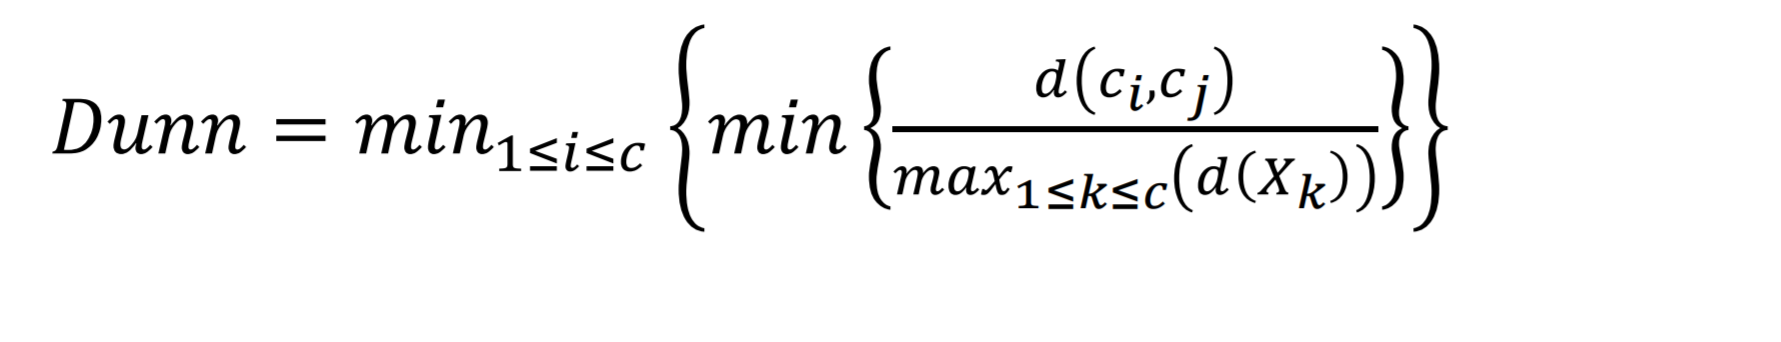
\includegraphics[width=0.7\textwidth]{images/dunn.png}
    
While $d(c_{i},c_{j}$) defines the intercluster distance between cluster $d(X_{i},X_{j}$) represents the intracluster distance of cluster $X_{k}$. \newline
$C$ is the number of cluster of data set.
Large values of index Dunn correspond to good clustering results, since higher values indicate that clusters are compact \cite{ballarin2015cluster}.The main disadvantage of the Dunn Index is that the calculation of the index is time consuming. Additionally, the index is very sensitive to noise, as the maximum cluster diameter can be large in a noisy environment \cite{ballarin2015cluster,rendon2011internal}. \newline

To sum up, the Dunn index can be computed with following steps [4]:\newline
    1.	For each cluster, compute the distance between each of the objects in the cluster and the objects in the other clusters \newline
    2.	Use the minimum of this pairwise distance as the inter-cluster separation (min.separation) \newline
    3.	For each cluster, compute the distance between the objects in the same cluster. \newline
    4.	Use the maximal intra-cluster distance (i.e maximum diameter) as the intra-cluster compactness \newline
    5.	Calculate the Dunn index (D) as follow: \newline

    D = $\frac{min.separation}{max.diameter}$ \cite{dunn-website-2} \newline

If the result shows compact and well-separated clusters the diameter of the clusters is expected to be small and the distance between the clusters is expected to be large. For our evaluation we use the implementation from \gls{sklearn}.

%%%%%
%The Dunn Index (in short DI) is a metric for evaluating clustering algorithms. Its aim is to identify sets of clusters \cite{dunn2016rizzo}. It is used for measuring an internal validation of clustering results \cite{BENNCIR2021102751}. \newline

%For each cluster, compute the distance between each of the objects in the cluster and the objects in the other clusters. Use the minimum of this pairwise distance as the inter-cluster separation (min. separation). For each cluster, compute the distance between the objects in the same cluster. Use the maximal intra-cluster distance (i.e maximum diameter) as the intra-cluster compactness. Calculate the Dunn index (D) as follow: \newline

%D = $\frac{min.separation}{max.diameter}$ \cite{BENNCIR2021102751} \newline

%The higher the value of the resulting Dunn index, the better the clustering result is considered, since higher values indicate that clusters are Compact. That means the greater the better \cite{dunnblog2019rizzo}.

\subsection{Calinski-Harabasz Index}
\textit{written by B.L.}\\

The Calinski-Harabasz criterion \cite{calinski1974dendrite} is defined as a proportional measure of within cluster variance to between cluster variance. That is why it is also known as the \gls{VRC}. Mathematically, this means
\begin{equation}
        CH = \frac{S_{B}}{S_{W}}\frac{m-K}{K-1} = \frac{\sum_{k=1}^{K} \left | C_{k} \right | \left \| c_{k} - \frac{1}{\left | X \right |}\sum_{x' \in X}^{} x' \right \|^{2}}{\sum_{k=1}^{K}\sum_{x \in C_{k}}^{} \left \| x - c_{i} \right \|^{2}} \frac{m-K}{K-1}
\end{equation}
utilizing the same notation as equation \ref{eq:kmeans_basic_other}. Between-cluster variance is divided by within-cluster variance. Dividing the data into more partitions of course reduces within-cluster variance, which is why there is also a scaling factor (second fraction representing degrees of freedom) to account for it. In comparison to \gls{DB} between-cluster variance is calculated in relation to the center of the data set in place of between individual cluster centers themselves. There is no upper limit to the value that can be achieved. A higher value is considered to be better.

Due to its construction (distance measure), this index performs well when clusters form mostly convex shapes. This can lead to mis-evaluation if the underlying data does not contain such globular clusters so a method capturing this might score lower while actually fitting the data better. It may therefore be better suited to compare different parameters for the same algorithm instead of comparing different algorithms. A comparative study of 30 cluster validation indices \cite{arbelaitz2013extensive} ranks \gls{CH} performance in evaluating fit near the top in many applications, particularly when evaluating K-Means results as expected.
    
    
\subsection{Davies-Bouldin Index}
\textit{written by J.M.}\\

%Davies-Bouldin \cite{davies1979cluster} brief explanation and reasons.
The Davies-Bouldin index is a metric to evaluate clustering algorithms and it was developed by David Davies and Donald Bouldin in 1979 \cite{davies1979cluster}. 
It is used to check the validity of clusters. To reach this, the Davies-Bouldin Index tries to maximize the inter-cluster distance 
and on the other side tries to minimize the intra-cluster distance. 
The Davies-Bouldin index is defined as \cite{davies1979cluster} 

\begin{equation}
	\bar{R} \equiv \frac{1}{N} \sum_{i=1}^{N} R_i  
\end{equation}
where N is the number of cluster and $R_i$ is the maximum of $R_{ij}$ where i$\neq$j 
\begin{equation}
	R_{ij} \equiv \frac{S_i+ S_j}{M_{ij}} \\
\end{equation}
where $M_{ij}$ is the Minkowski metric which can be descibes as: 
\begin{equation}	
	M_{ij} = \{ \sum_{k=1}^{N} |a_{ki} - a_{kj}  |^p    \} ^{  \frac{1}{p}}    	
\end{equation}
\begin{equation}
	S_{ij} = \{\frac{1}{T_i} \sum_{j=1}^{T_i} |X_{j} - A_{i}  |^q    \}^\frac{1}{q} 
\end{equation}
	
If q =1 	$S_{ij}$ is the Euclidean distance between centroids.  \\
  
For our evaluation we use the implementation from sklearn of this metric. This metric calculates a score. Zero is the lowest score that can be reached. If a score is closer to zero, it relates to a better separation between the calculated clusters. 

\subsection{Silhouette Score}
\label{Silhouette Score}
\textit{written by L.B.}\\

Cluster validation indexes are used to assess clustering quality. That means it is investigated whether the resulting clusters reflect natural structures in the data or whether clusters rather determine artificial groups. In general, the ratio of dissimilarity between data points within the same cluster to dissimilarity between data points in different clusters is a measurement for clustering quality. 
The Silhouette Score is one of such cluster validation indexes which can be applied to evaluate clustering results if Euclidean distance measures can be calculated on the underlying data set. According to that, a clustering result as well as proximity scores between all data points have to be provided to be able to compute the Silhouette Score. 
For a single data point, distances to all the data points assigned to the same cluster are calculated. Here, the mean of all these distances is called \textit{a}. After that, the nearest cluster for each data point has to be identified. This can be done by iteratively calculating the mean of distances between the single data point and all data points within another cluster until distances for all clusters have been computed. The minimum average distance determines the nearest cluster for the single data point. 
The minimum average distance is called \textit{b} here. The Silhouette Score for data point \textit{i} is calculated using the following formula:
\begin{align*}
	s(i)=\frac{b - a}{max(a, b)}.
\end{align*}
The mean of all the Silhouette Scores for each individual data point determines the Silhouette Score for the whole data set. As the nearest cluster has to be found for each of the included data points, the Silhouette Score can only be computed as soon as more than one cluster exists \cite{rousseeuw1987silhouettes}.
Taking a closer look at extreme cluster results determines how to interpret the Silhouette Score values: Given a partition where the mean intra-cluster distance \textit{a} is extremely low while the mean inter-cluster distance \textit{b} is high, the Silhouette Score would tend to be \mintinline[bgcolor=code-bg]{python}{1}. Hence, a Silhouette Score of \mintinline[bgcolor=code-bg]{python}{1} corresponds to a well-partitioned data set because the mean of distances between single points and other clusters than the one it is assigned to is large. Analogously, a value of \mintinline[bgcolor=code-bg]{python}{-1} corresponds to a partition where the inter-cluster distance \textit{b} is much smaller than the intra-cluster distance \textit{a}. Thus, the data points are not assigned to their nearest clusters, resulting in a mis-classification. If the Silhouette Score is equal to zero, means of inter- and intra-cluster distances are close to each other and it is unclear which cluster the point should have been assigned to. In this case, the partition can also contain overlapping clusters \cite{rousseeuw1987silhouettes}.
For the calculation of Silhouette Scores, we utilize the implementation provided by sklearn \cite{sklearn_api}.
We decided to use of the Silhouette Score as it can be applied on cluster results generated with any clustering technique. It therefore provides an intuitive way of comparing the results of different algorithms to each other. In addition to that, Silhouette Scores are relatively easy to interpret, given that there is a maximum and a minimum score that can be reached. One disadvantage is that Silhouette Scores are higher for convex clusters. As some density-based clustering algorithms like Mean Shift or Spectral Clustering explicitly allow the creation of non-convex clusters, the obtained Silhouette Scores could possibly be lower than results created applying other clustering techniques.
%\item Gap \cite{tibshirani2001estimating} brief explanation and reasons.

\subsection{Results}

In the following there is a discussion of the results of all clustering efforts in detail. A brief overview of the evaluation results can be found in table \ref{tab:evalutaion_table}. For each data set there is a row for each algorithm used. In columns are the results for each index. The cells represent the highest (lowest for \gls{DB} respectively) value achieved by applying various parameter configurations. It should be noted that comparing results across different methods does not show the entire picture but it can yield indications on performance.

\begin{table}[H]
\begin{center}
%\resizebox{\textwidth}{!}{%
\begin{tabular}{lrrrr}
Data and Method & \multicolumn{1}{c}{\gls{CH}} & \multicolumn{1}{c}{\gls{DB}} & \multicolumn{1}{c}{\gls{SI}} & \multicolumn{1}{c}{\gls{DI}} \\ \hline
 &  &  &  &  \\
\textbf{Housing} &  &  &  & \\
K-Means & 1621.90 & 0.326 & 0.721 & 0.525 \\
Mean Shift & 1338.65 & 0.326 & 0.721 & 0.111 \\
Affinity & 1803.31 & 0.350 & 0.372 & 0.185 \\
Spectral & 1456.86 & 0.546 & 0.689 & 0.525 \\
 &  &  &  &  \\
\textbf{Mall} &  &  &  &  \\
K-Means & 301.02 & 0.766 & 0.479 & 0.843 \\
Mean Shift & 921.29 & 0.103 & 0.438 & 0.905 \\
Affinity & 314.89 & 0.282 & 0.371 & 0.382 \\
Spectral & 262.82 & 0.731 & 0.454 & 0.087 \\
 &  &  &  &  \\
\textbf{Seeds} &  &  &  &  \\
K-Means & 369.55 & 0.691 & 0.492 & 0.091 \\
Mean Shift & 374.19 & 0.689 & 0.519 & 0.113 \\
Affinity & 374.12 & 0.642 & 0.529 & 0.086 \\
Spectral & 335.58 & 0.638 & 0.525 & 0.107 \\
 &  &  &  &  \\
\textbf{Wine} &  &  &  &  \\
K-Means & 3116.82 & 0.617 & 0.603 & 0.049 \\
Mean Shift & 1346.44 & 0.366 & 0.768 & 0.079 \\
Affinity & 2633.03 & 0.927 & 0.261 & 0.041 \\
Spectral & 2616.13 & 0.668 & 0.534 & 0.007
\end{tabular}%
%}
\end{center}
\caption{Comparing All Algorithms On All Data Sets For All Evaluation Indices}
\label{tab:evalutaion_table}
\end{table}


\subsubsection{Seeds - K-Means}
\textit{written by B.L.}\\
\label{sec:seeds_kmeans_evaluation}

\begin{table}[H]
\begin{center}
%\resizebox{\textwidth}{!}{%
\begin{tabular}{crrrr}
$K$ & \multicolumn{1}{c}{\gls{CH}} & \multicolumn{1}{c}{\gls{DB}} & \multicolumn{1}{c}{\gls{SI}} & \multicolumn{1}{c}{\gls{DI}} \\ \hline
2 & 351.235 & 0.688 & 0.519 & 0.038 \\
3 & 375.804 & 0.753 & 0.471 & 0.085 \\
4 & 327.439 & 0.825 & 0.412 & 0.020 \\
5 & 310.331 & 0.915 & 0.361 & 0.091 \\
6 & 302.344 & 0.917 & 0.366 & 0.106 \\
7 & 294.385 & 0.939 & 0.350 & 0.077 \\
8 & 297.502 & 0.937 & 0.362 & 0.083 \\
\end{tabular}%
%}
\end{center}
\caption{K-Means Seeds Data Set Indices by Number of Clusters}
\label{tab:kmeans_seeds_table}
\end{table}

Table \ref{tab:kmeans_seeds_table} contains the index scores for each of the indices selected as columns and the number of clusters as rows. An easier representation of this data is a line chart which can be seen in Figure \ref{fig:kmeans_seeds_comparison_plot} and in the following description of results. More than simply a tool to compare scores between methods, these can help in identifying the number of clusters (or other parameters below) best fit to represent the data. So what can be learned from the data: If there is a clear maximum (minimum for \gls{DB}) value for an index it indicates looking at that value to gain insight on the fit. If there is no clear maximum (minimum) value, one can try to employ the so called elbow criterion (see section \ref{subsec:method_kmeans}) where a distinct change in direction for a graph might indicate a value worth examining. If there is neither there seems to be no information gain at hand from that particular index for this application.

\begin{figure}[H]
\centering
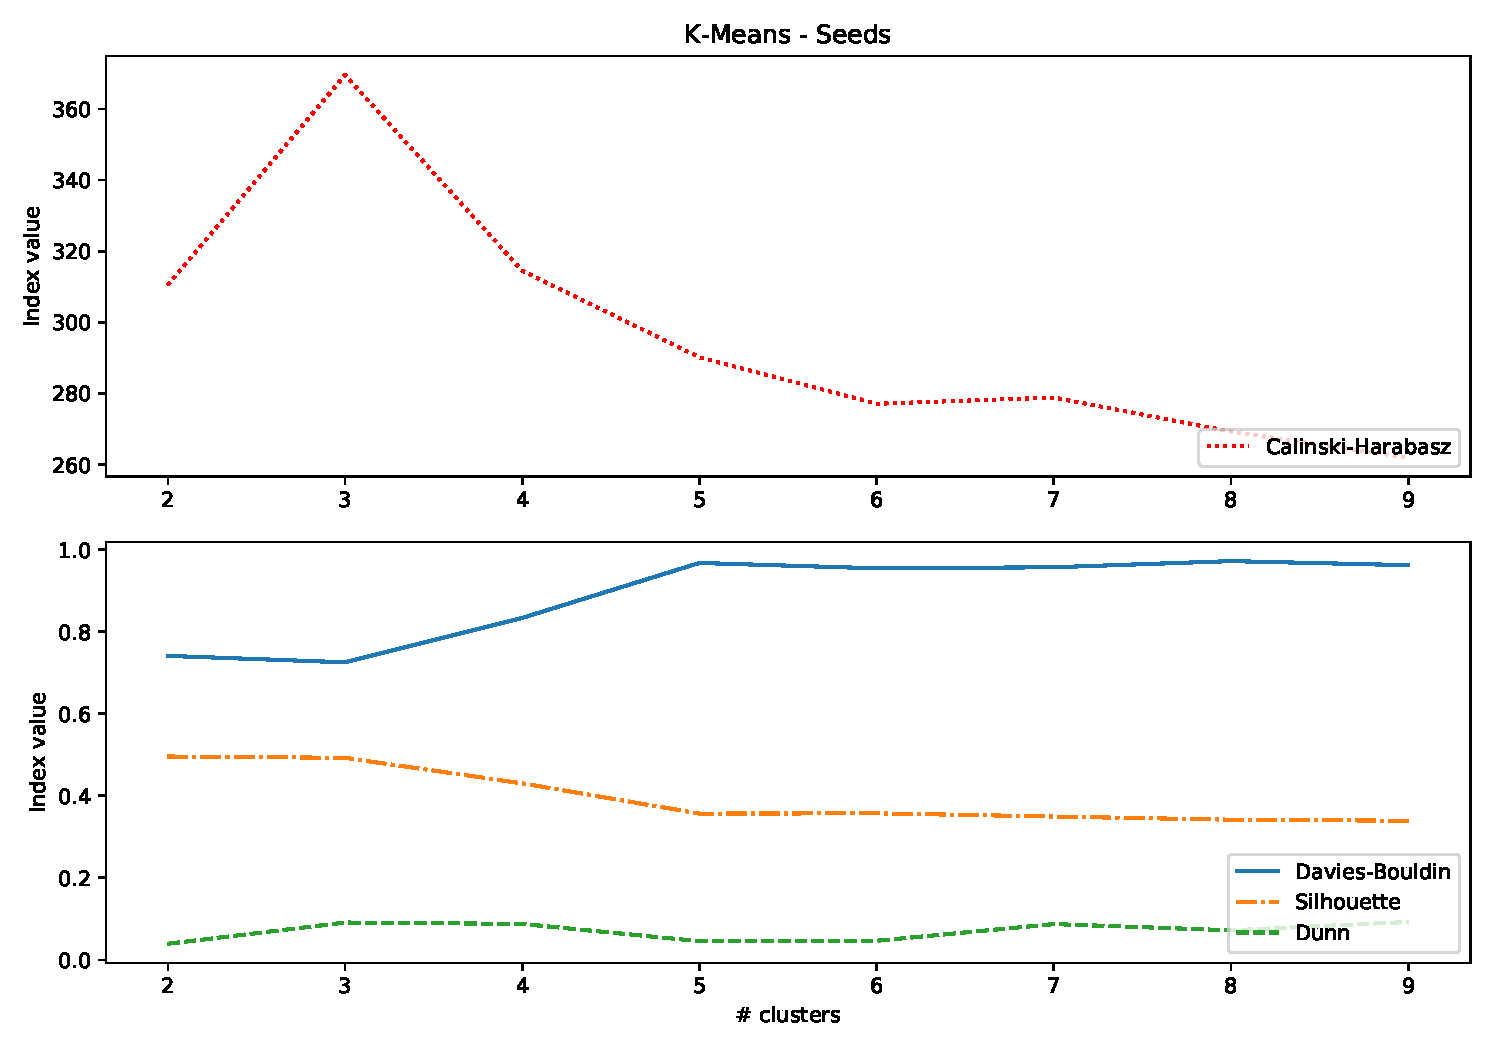
\includegraphics[width=1.0\textwidth]{images/kmeans_seeds_index_plot.pdf}
\caption{K-Means Seeds Data Set Indices by Number of Clusters}
\label{fig:kmeans_seeds_comparison_plot}
\end{figure}

\vspace{-0.5cm}
Looking at Figure \ref{fig:kmeans_seeds_comparison_plot} (one line for each index, two panels because of the vastly different scale of \gls{CH}) one can see a clear maximum in \gls{CH} value and a local maximum in \gls{DI} as well as a change in slope for \gls{SI} at three clusters each. Following the described logic, \gls{DB} also suggests considering three clusters. 

As mentioned in section \ref{sec:data_description} this data set originally comes with labels which allows to use them as a benchmark to see how the clustering performs. Plotting (Figure \ref{fig:kmeans_seeds_tsne}) two dimensional representations (see t-SNE in section \ref{sec:frontend_description}) of the K-Means clustered result next to the original data shows a few things: the algorithm has, as expected, produced non-overlapping mostly contiguously shaped clusters in contrast to the original data. However using three clusters has generally produced a reasonably good fit, as is supported by an accuracy of 89.5\%, precision of 90\% and recall of 89.5\% to name a few common metrics.

\begin{figure}[H]
\begin{center}
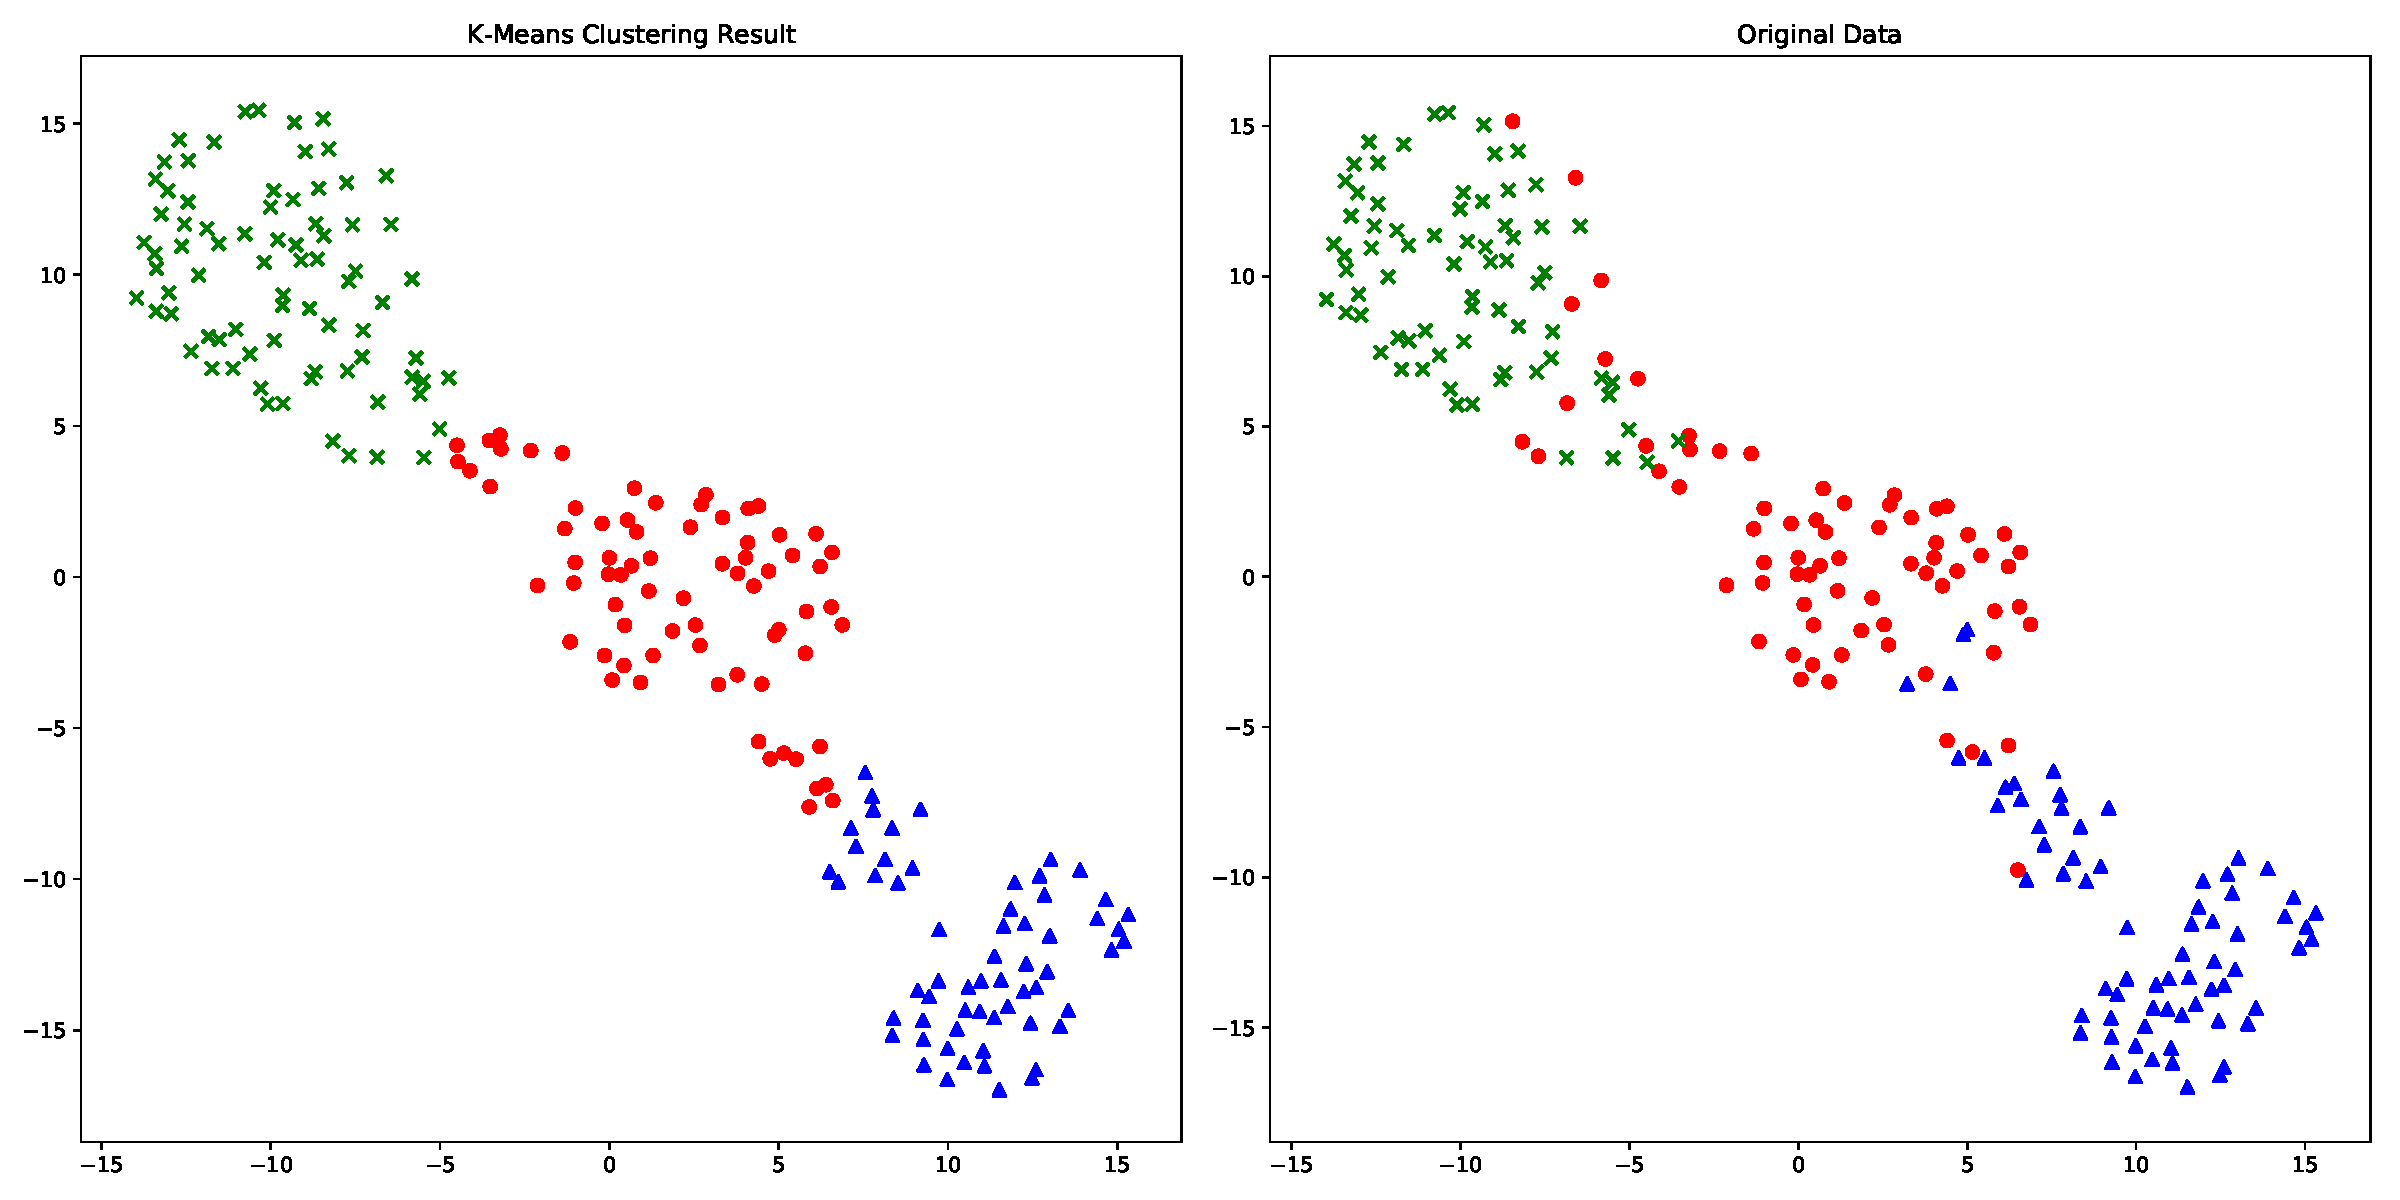
\includegraphics[width=1.0\textwidth]{images/kmeans_seeds_tsne.pdf}
\end{center}
\caption{Seeds Data Set Comparison Clustering and Original Labels}
\label{fig:kmeans_seeds_tsne}
\end{figure}

%continuous data in all features makes application straight forward
%as shown in table \ref{tab:k-means_seeds_table} data on how many clusters to choose not clear
%looking at chart in \ref{fig:kmeans_seeds_indices_plot} makes comparison easier. shows \gls{CH} with significant signal at three clusters and \gls{DI} flattening out after three clusters while \gls{SI} falling after three clusters. only \gls{DB} highest at seven clusters. in light of this analysis it doesn't seem unreasonable to select three clusters as the best fit. looking at the data in 3d, see figure

\subsubsection{Seeds - Mean Shift}
\textit{written by L.B.}\\ 

In the following two plots, values for the chosen cluster validation indexes that evaluate the clustering result generated applying the Mean Shift algorithm on the Seeds data set for a range of bandwidth parameters are provided (Figure \ref{fig:mean_shift_seeds_indexes}).
To determine suitable bandwidth parameter values, ideally \gls{SI}, \gls{DI} and \gls{CH} should be maximized while \gls{DB} should be at a minimum. 
Reaching this goal is not that easy due to the way those scores are computed.
\newline
\begin{figure}[H]
\begin{center}
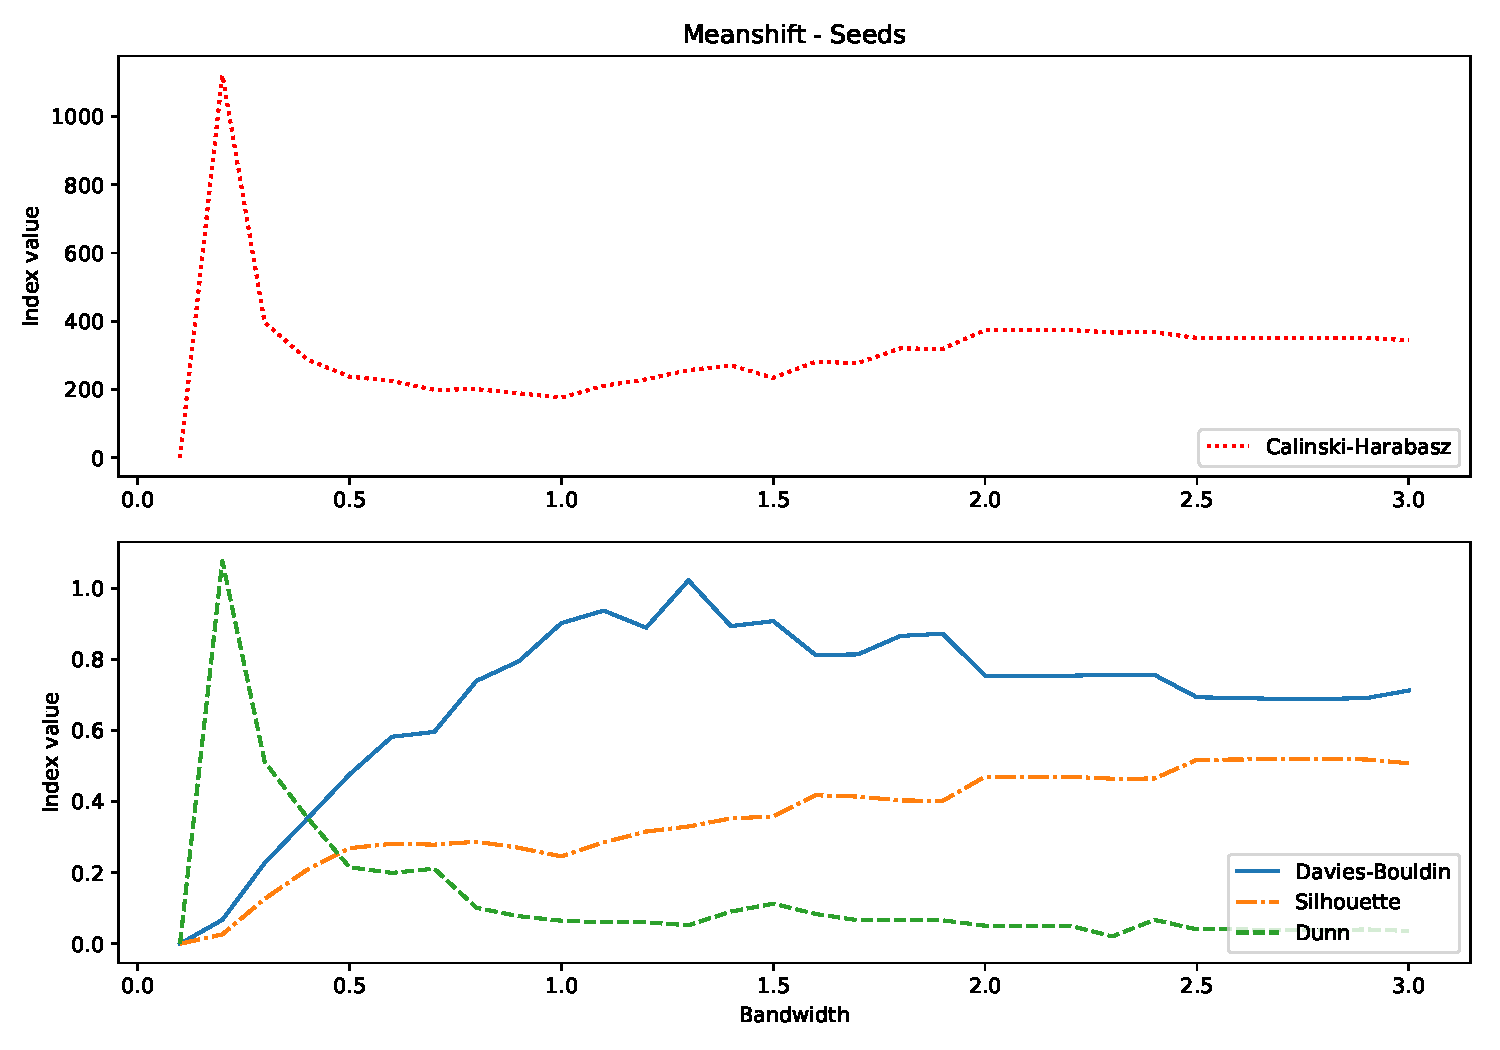
\includegraphics[width=0.8\textwidth]{images/Meanshift_-_Seeds.pdf}
\end{center}
\caption{Cluster Validation Indexes: Means Shift on Seeds}
\label{fig:mean_shift_seeds_indexes}
\end{figure}
Taking a look at \gls{DI}, \gls{CH} and \gls{DB}, one might choose a bandwidth of 0.2 which indeed results in a very high number of small clusters and does not seem to represent a natural structure within the data set as can be seen in Figure \ref{fig:meanshift_seeds_clustering_tsne}.
\begin{figure}[H]
    \centering
    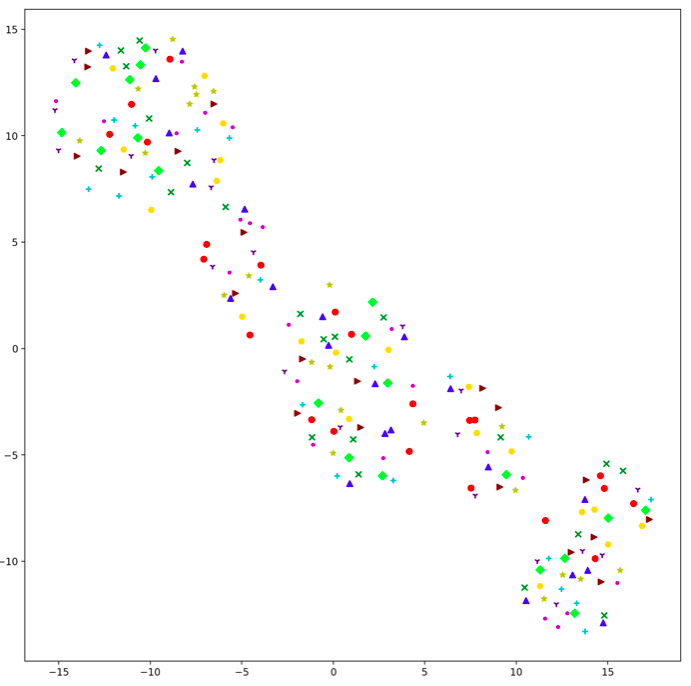
\includegraphics[width=0.5\textwidth]{images/Meanshift_Seeds_0_2.png}
    \caption{t-SNE projected result of Mean Shift with bandwidth = 0.2 on Seeds data set}
    \label{fig:meanshift_seeds_clustering_tsne}
\end{figure}

Instead, a balance between high values for \gls{DI}, \gls{SI}, \gls{CH} and a low value for \gls{DB} is found for bandwidth values of 2 or 2.5 which results in two respectively three distinct clusters (Figure \ref{fig:meanshift_seeds_2_tsne}). 
\begin{figure}[H]
    \subfigure{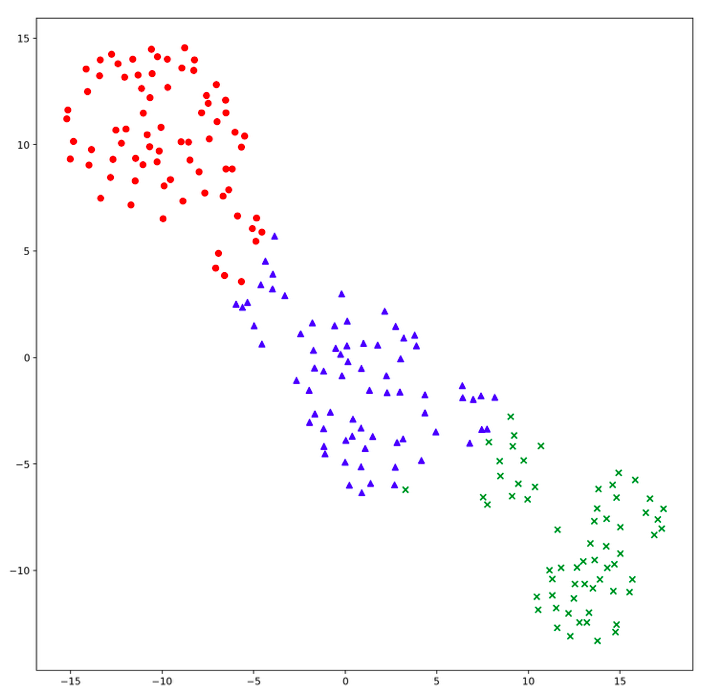
\includegraphics[width=0.49\textwidth]{images/Meanshift_Seeds_2.png}}
    \subfigure{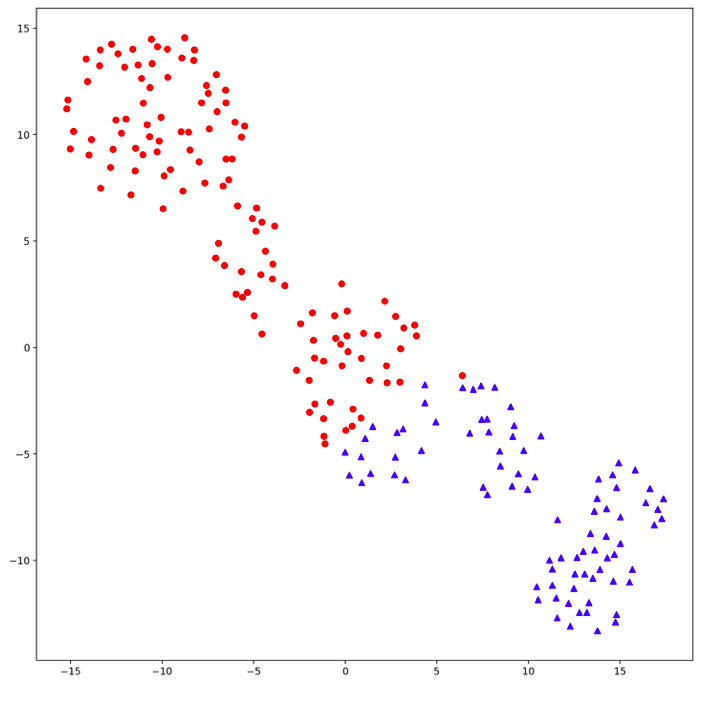
\includegraphics[width=0.49\textwidth]{images/Meanshift_Seeds_2_5.png}}
    \caption{t-SNE projected result of Mean Shift with bandwidth = 2 (left) and bandwidth = 2.5 (right) on Seeds data set}
    \label{fig:meanshift_seeds_2_tsne}
\end{figure}

As the data set is labeled (see section \ref{sec:seeds_kmeans_evaluation}), a comparison with the original labels would probably support choosing a bandwidth parameter value of 2.

\subsubsection{Seeds - Affinity Propagation}
\textit{written by J.M.}\\

\begin{figure}[H]
	\begin{center}
		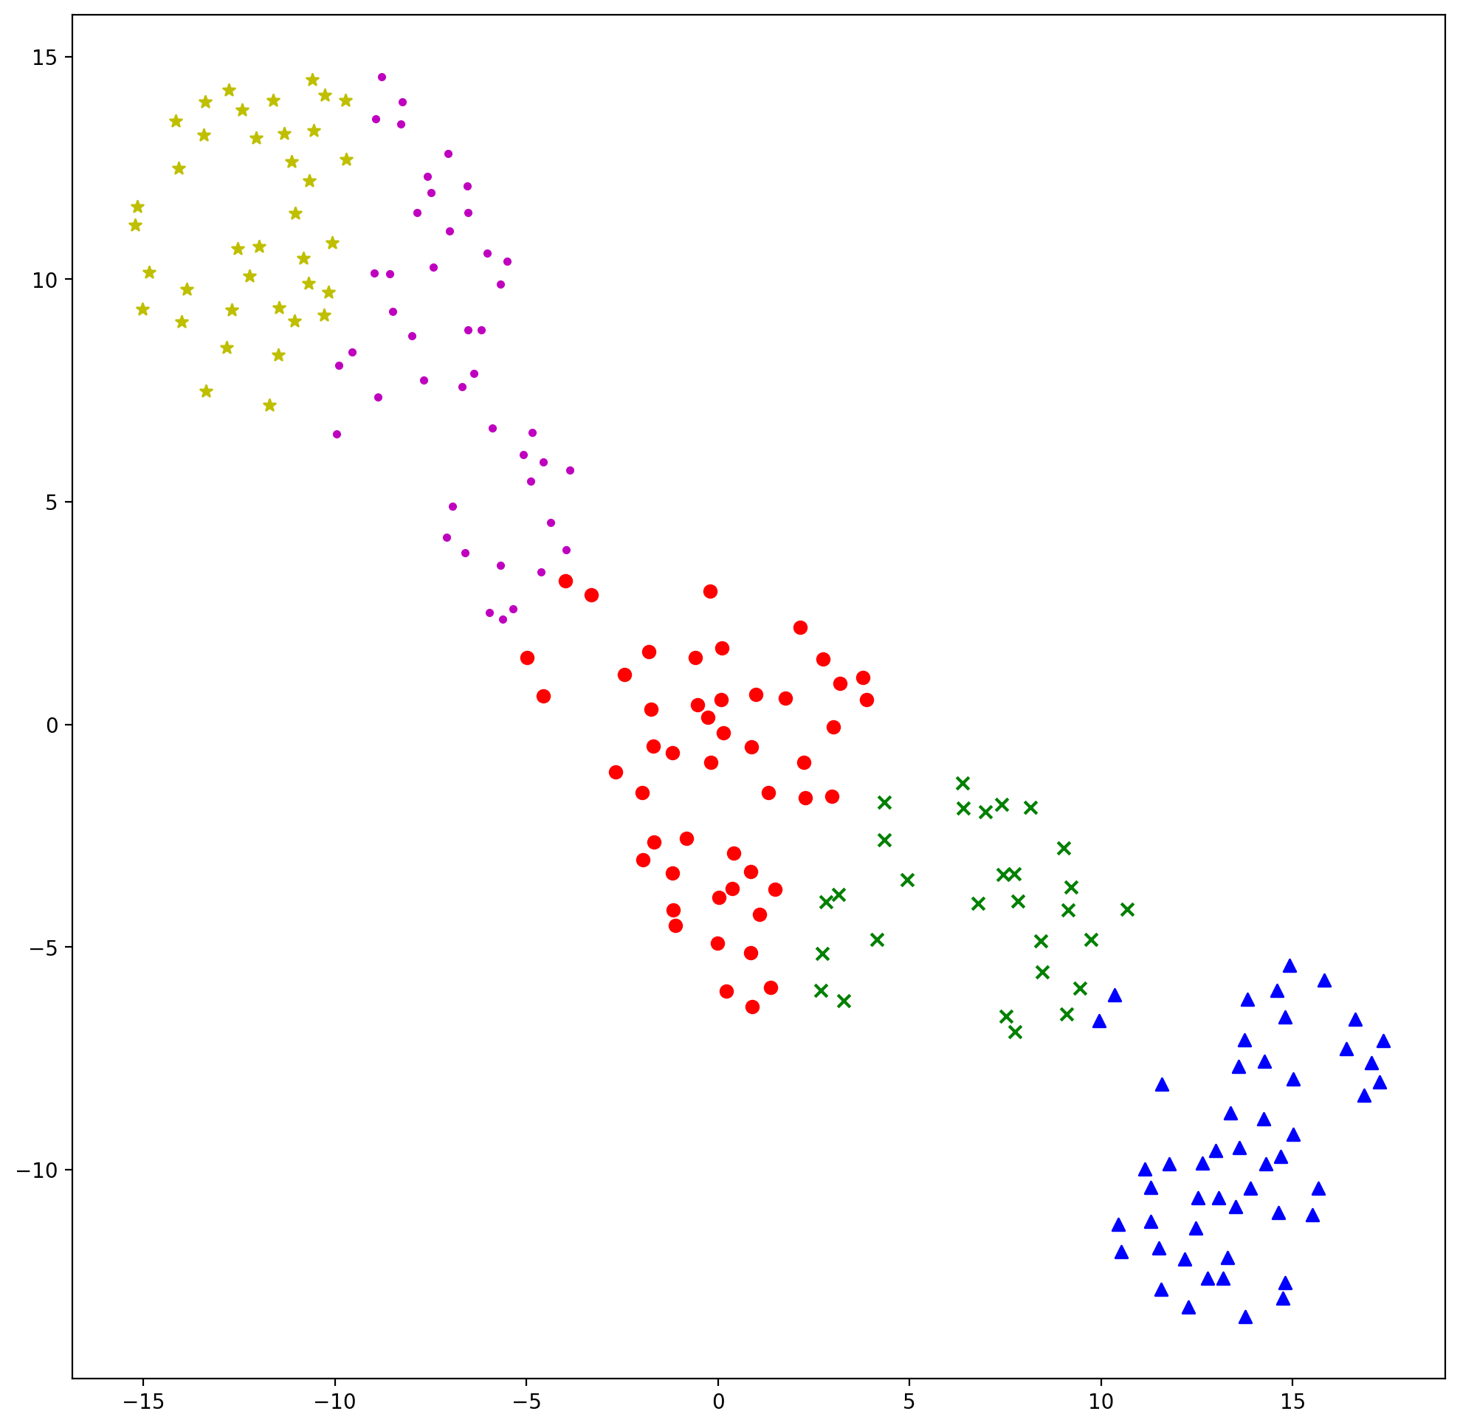
\includegraphics[width=0.5\textwidth]{images/af_seed78.png}
	\end{center}
	\caption{t-SNE plot of Affinity Propagation on Seeds data set}
	\label{fig:af_seeds78}
\end{figure}

\begin{figure}[H]
	\begin{center}
		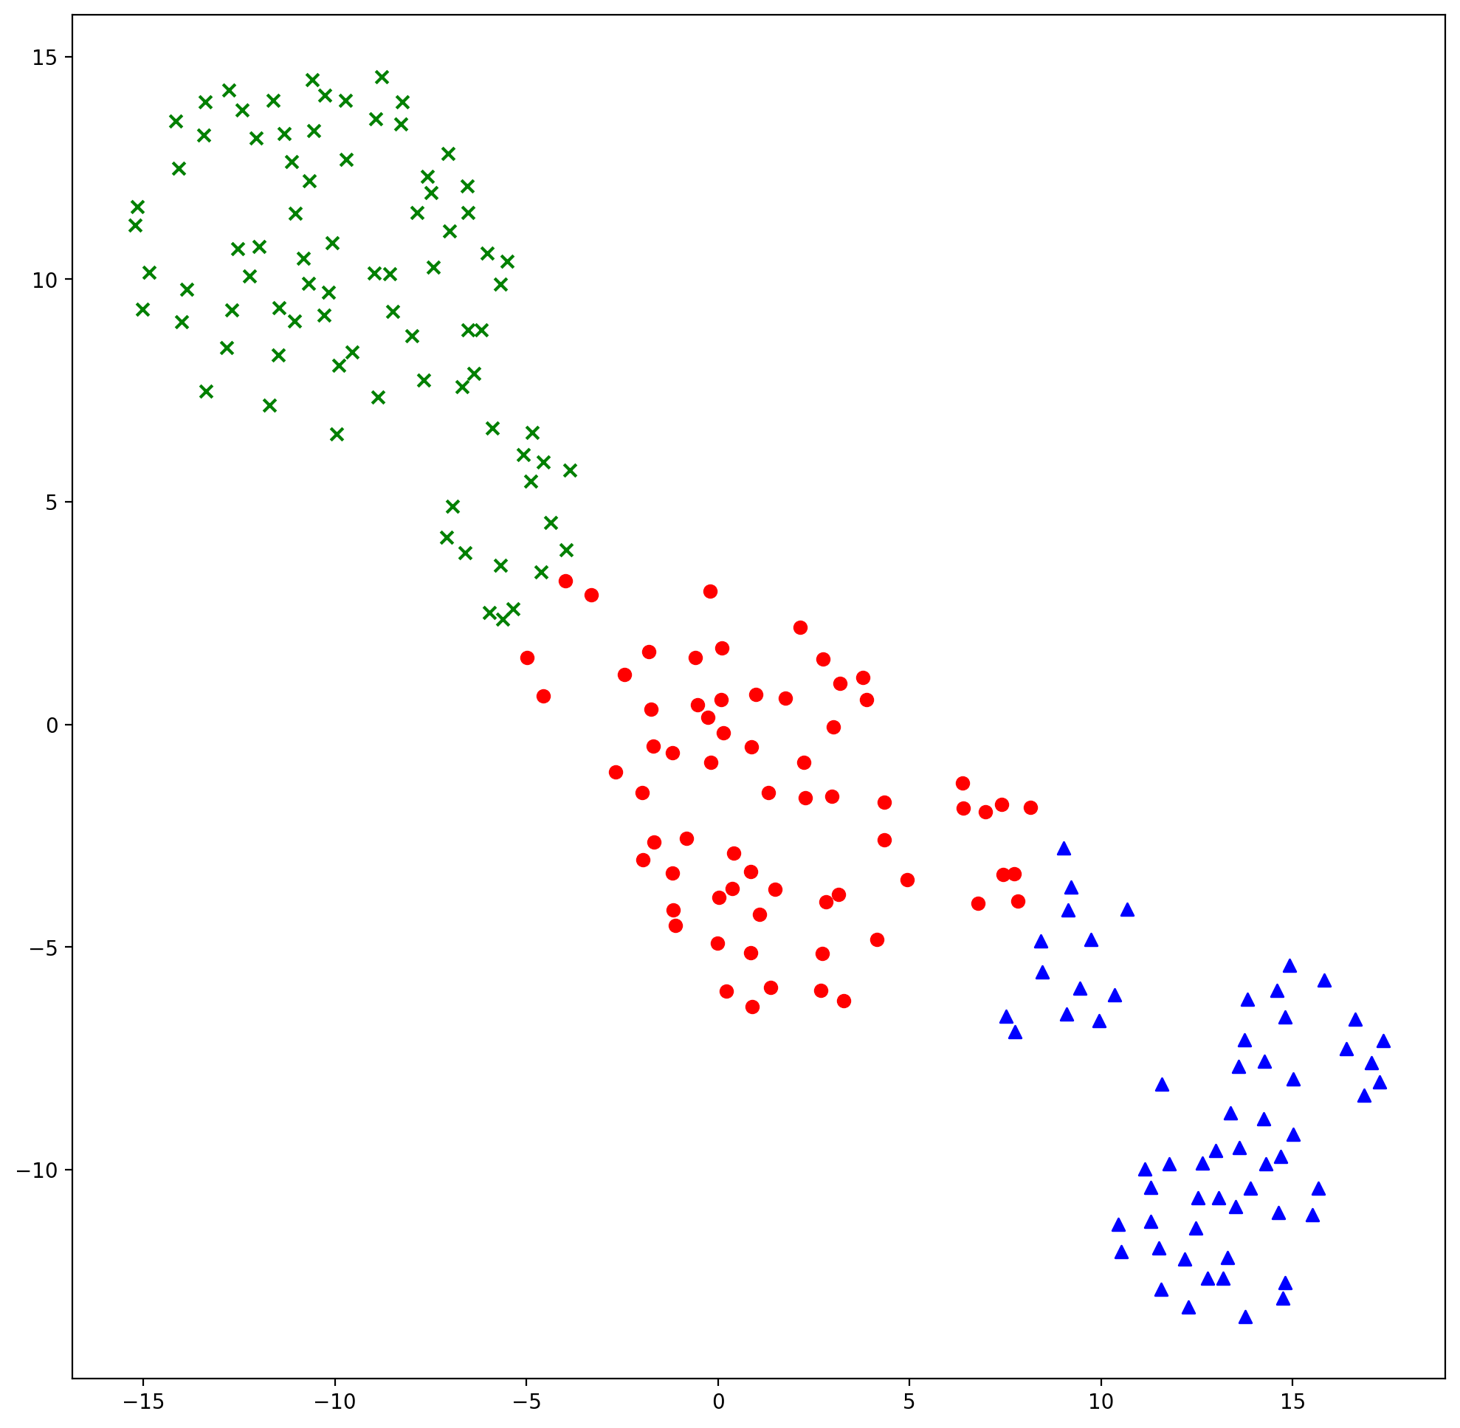
\includegraphics[width=0.5\textwidth]{images/af_seeds247.png}
	\end{center}
	\caption{t-SNE plot of Affinity Propagation on Seeds data set}
	\label{fig:af_seeds2}
\end{figure}

On the Seeds data set it performs good. And it finds some good clusters. Depending on the parameter, more or less clusters are created which are shown in Figure \ref{fig:af_seeds78} and Figure \ref{fig:af_seeds2}. In Figure \ref{fig:af_seeds78}, the input parameter is -78. It is very low compared to the parameter that are used for the other data sets. If this parameter gets lower, Affinity Propagation will create less clusters like in Figure \ref{fig:af_seeds2}. Here, the parameter is -247. If you compare the cluster validation metrics on these two plots, you can see that the second plot is better in all cluster validation metrics. If we look to other parameters, we do not find new insights, the parameter -247 is quite optimal for this data set. 
\begin{table}[H]
	\centering
	\begin{tabular}{||c c c ||} 
		\hline
		cluster validation & plot1 & plot2 \\ [0.5ex] 
		\hline\hline
		Calinski-Harabasz & 302.7425	 &  374.6137  \\ 
		Davies-Bouldin & 0.8784	 & 0.7544	 \\
		Silhouette & 0.3644	 & 0.4681	 \\
		Dunn & 0.0489 & 0.0495  \\ [1ex] 
		\hline
	\end{tabular}
	\caption{Comparison Cluster validation Affinity Propagation}
	
\end{table}

\subsubsection{Seeds - Spectral Clustering}
\textit{written by M.A.}

Cluster validation indices are applied and compared to the respective datasets. The indices SI, DI, and CH are optimal when they reach the maximum. DB reaches the optimal value with a minimum. To compare the scores between different methods, the following line chart in Figure 13 is being analysed identifying the number of dimensions of the projection subspace for the Seeds data set. \newline

\begin{figure}[H]
    \centering
    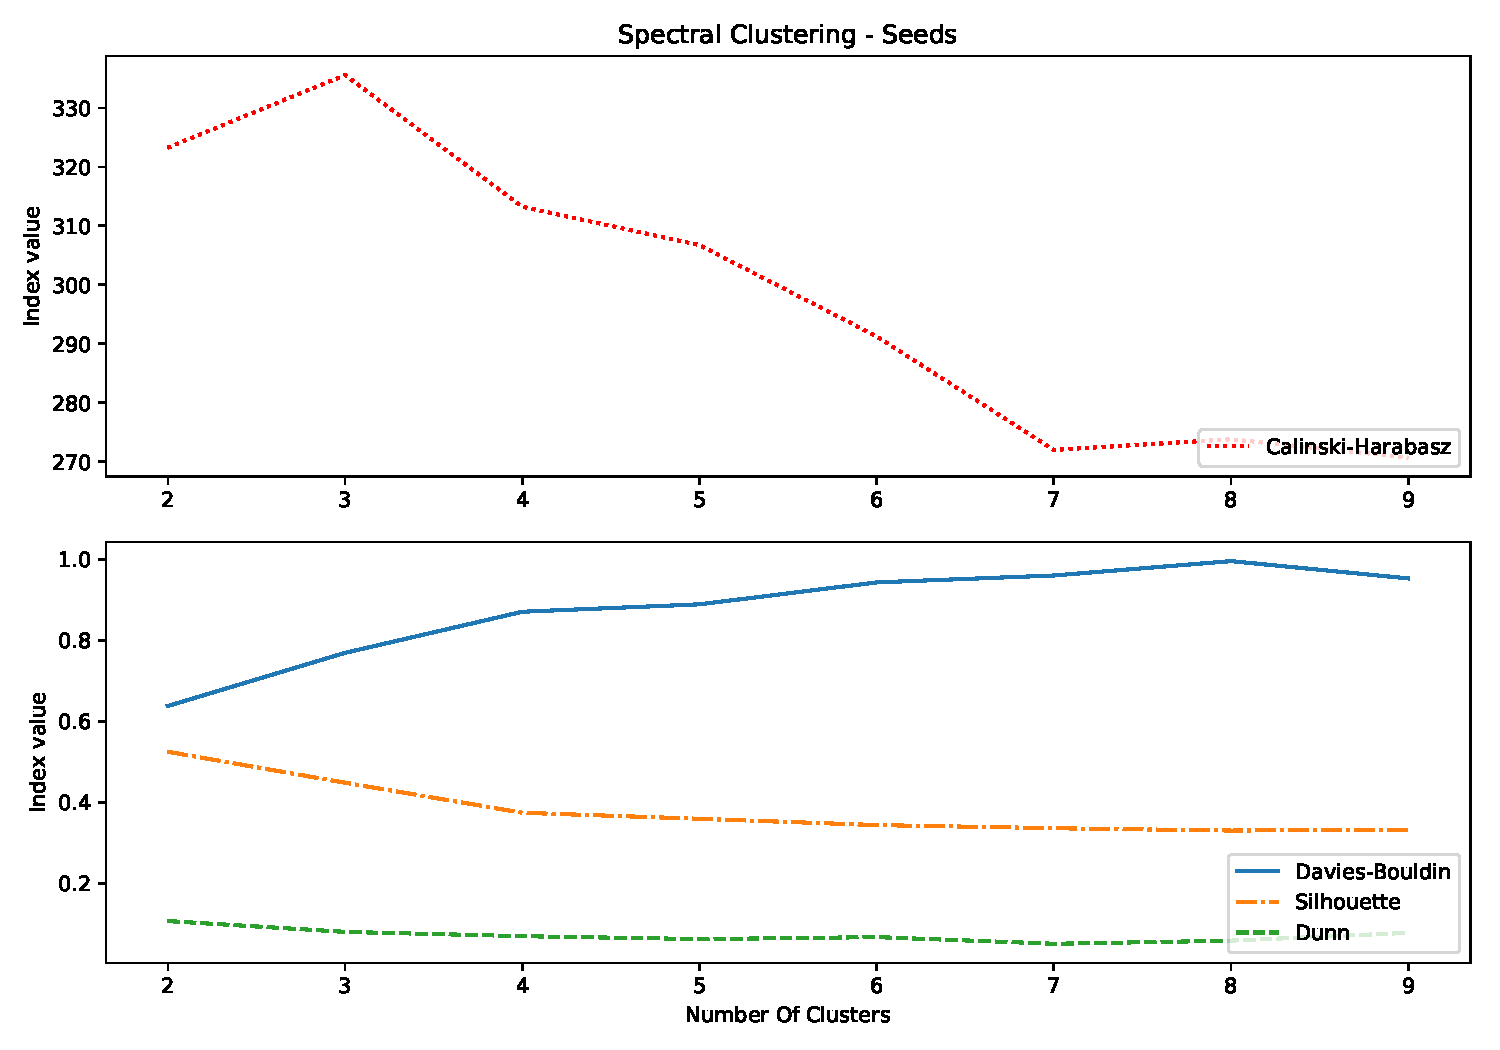
\includegraphics[width=1\textwidth]{images/Spectral_Clustering_-_Seeds.pdf}
    \caption{t-SNE projected result of Spectral Clustering with dimension = 2}
    \label{fig:my_label}
\end{figure}
% \newline

%Figure 1: Cluster validation indices by number of dimensions: Spectral Clustering on Seeds data set \newline

At first glance, one can determine the maximum of CH, which is being reached at 3 dimensions. On the other hand, SI and DI suggest 2 dimensions, which can be derived through the maximum located at 2. Even DB, which shows the best result in its minimal value suggests 2 dimensions, since the line rises from that point on. Figure 2 shows the result of Spectral Clustering for dimension 2.

\begin{figure}[H]
    \centering
    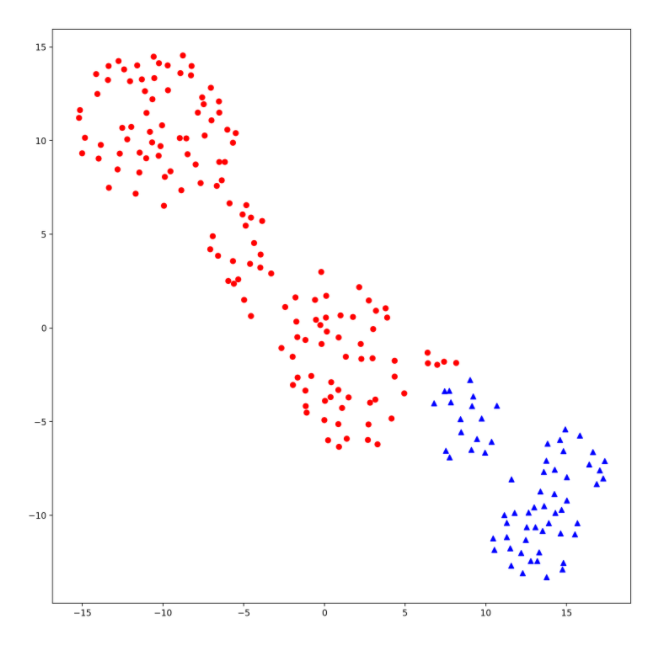
\includegraphics[width=0.5\textwidth]{images/k2.PNG}
    \caption{t-SNE projected result of Spectral Clustering with dimension = 2}
    \label{fig:my_label}
\end{figure}


\subsubsection{Mall Customers - K-Means}
\textit{written by B.L.}\\
\label{sec:mall_kmeans_evaluation}

\begin{wrapfigure}{r}{0.5\textwidth}
  \centering
    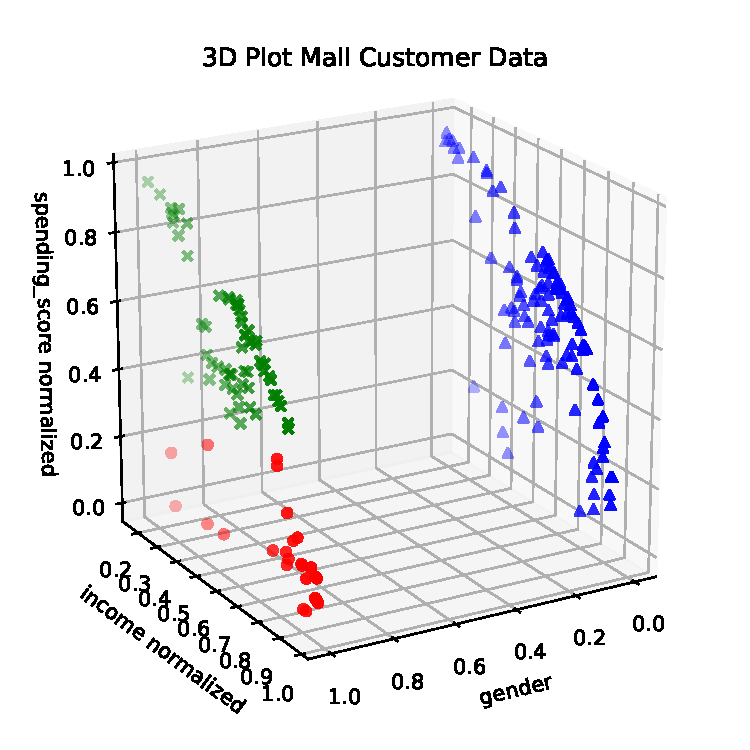
\includegraphics[width=0.48\textwidth, clip]{images/kmeans_customers_3d.pdf}
  \caption{Split Data Due To {Categorical} Feature}
  \label{fig:kmeans_customers_3d}
\end{wrapfigure}

As one of the features is categorical (gender), this is not an ideal application of the K-Means clustering method. The categories can be resolved into discrete values so that calculations can be run, but the arbitrary nature of this does not really allow for good interpretation of the results. An exemplary three dimensional plot in Figure \ref{fig:kmeans_customers_3d} shows the issue: 

gender is represented on the z-axis and the two manifestations simply rip the data into two partitions. When gender is encoded as 0 and 1, this showed almost no effect. When using 0 and 100, it leads to a doubling in the index-recommended number of clusters. One attempt to deal with this is to scale all data between 0 and 1 but this aggravated the problem instead of improving on it. Extensions of the K-Means method have been devised to deal with this type of data (as described in section \ref{subsec:method_kmeans}) but their application here seems beyond the scope of this work. Using the gender feature also does not improve scores in the evaluation methods used. Given these circumstances, considering plot \ref{fig:kmeans_customers_indices_plot} suggests considering the results for 2 (\gls{CH}, \gls{DB}, \gls{SI}), 7 (\gls{DB}) or 8 (\gls{CH}) clusters.

\begin{figure}[H]
\begin{center}
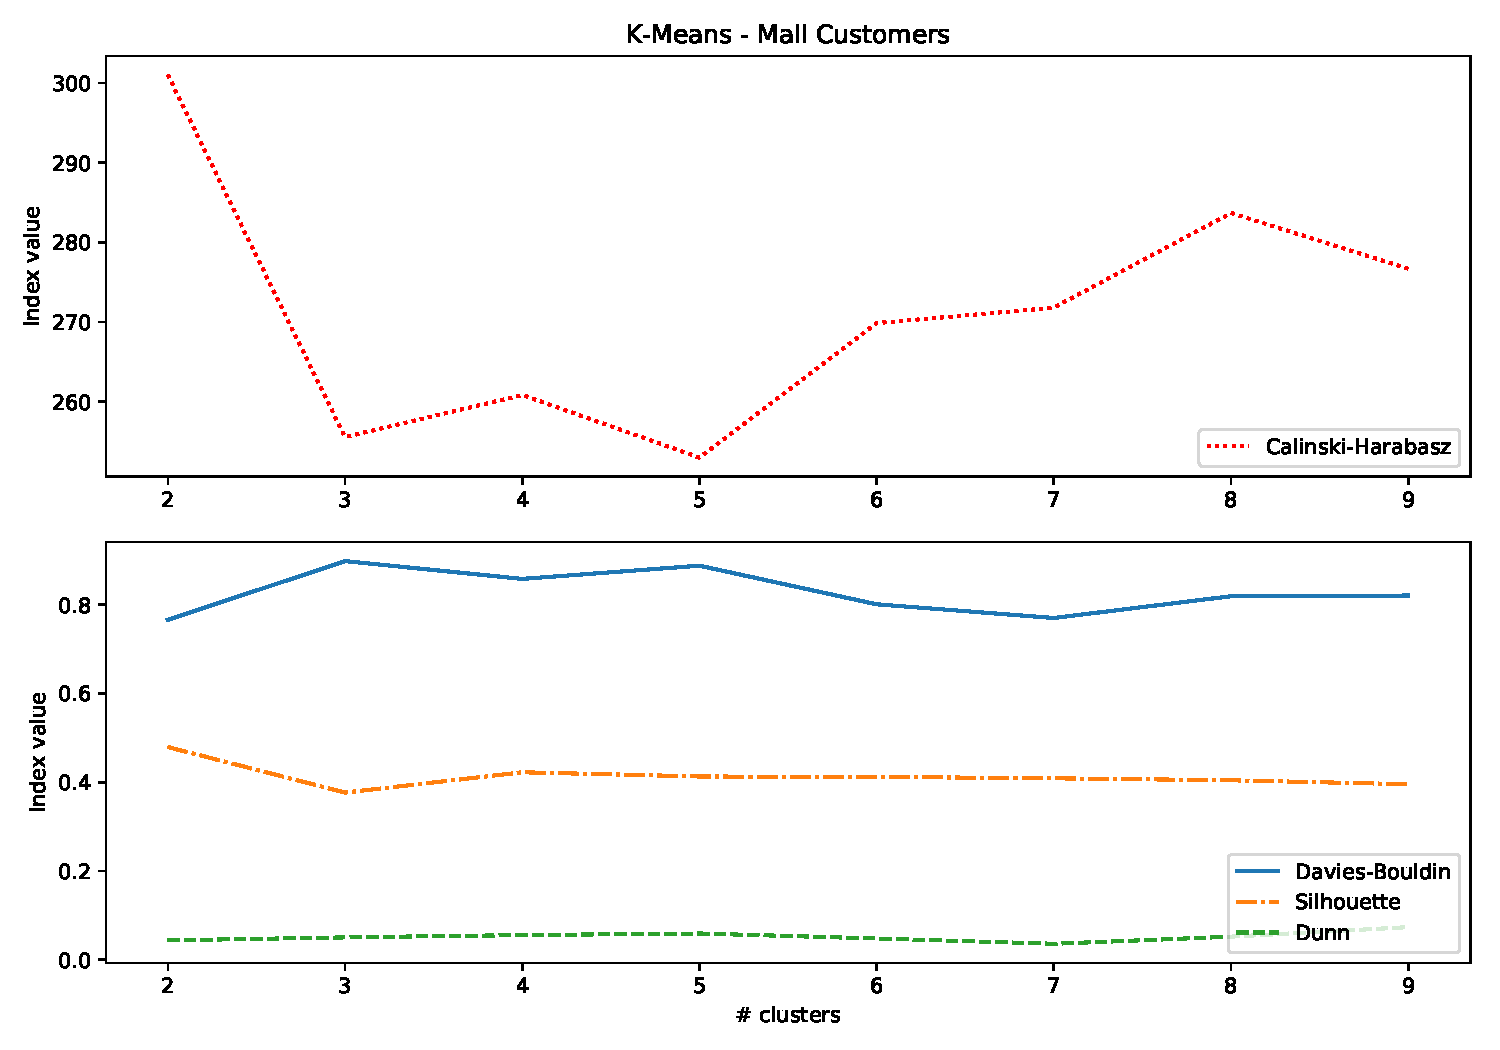
\includegraphics[width=1.0\textwidth]{images/kmeans_customers_index_plot.pdf}
\end{center}
\caption{K-Means Mall Customers Data Set Indices by Number of Clusters}
\label{fig:kmeans_customers_indices_plot}
\end{figure}

The data set contains four features, three of which have a measurable and interpretable impact on clustering, which lends itself to a visual comparison in three dimensional space. Figure \ref{fig:kmeans_customers_3d_multi} shows three plots, one for each suggested number of clusters. The highest overall evaluation scores were achieved for two clusters and purely from a visual standpoint this seems to be a solution holding some weight. 

\begin{figure}[H]
\begin{center}
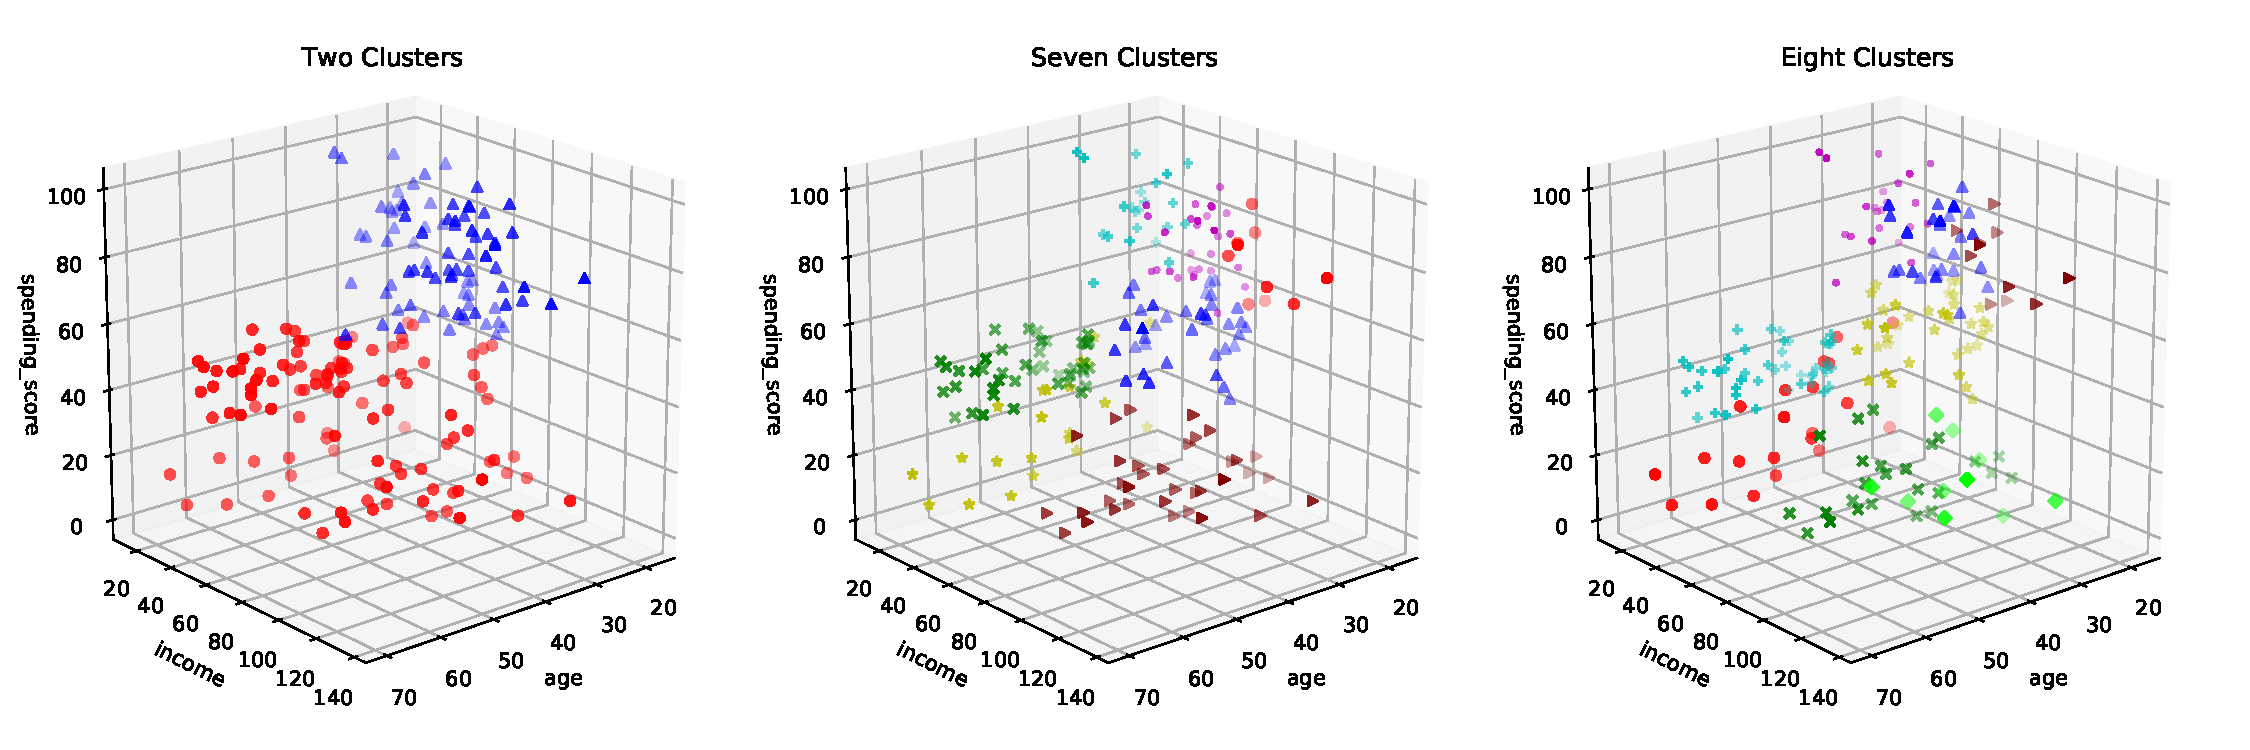
\includegraphics[width=1.0\textwidth]{images/kmeans_mall_3d_multi.pdf}
\end{center}
\caption{Mall Customers 3D Plot Clustering Options}
\label{fig:kmeans_customers_3d_multi}
\end{figure}
\vspace{-0.5cm}

%Rotating the plot shows that both partitions contain very similar clusters but due to the way K-Means works they are not recognized as the same. The data shows either two clusters (simply male cluster and female cluster) or an ideal number of clusters double the amount perceived by a human to be reasonable.

\subsubsection{Mall Customers - Mean Shift}
\textit{written by L.B.}\\

The influence of different bandwidth parameter values for the application of Mean Shift on the Mall data set can be seen in Figure \ref{fig:meanshift_mall}.

\begin{figure}[H]
\begin{center}
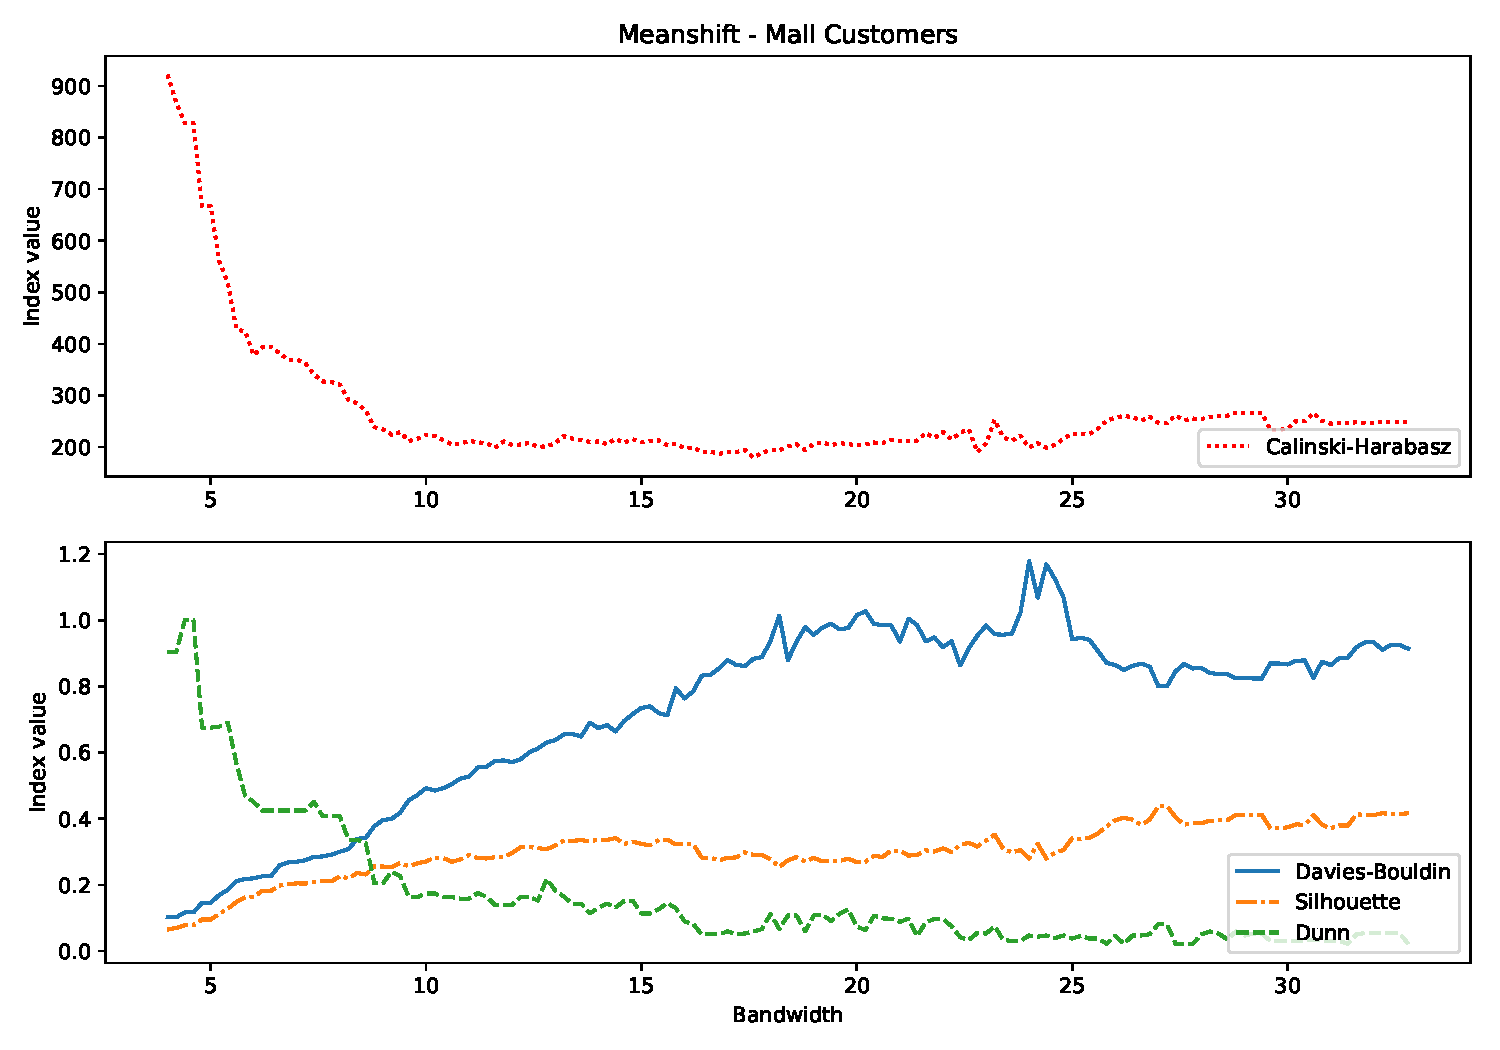
\includegraphics[width=0.8\textwidth]{images/Meanshift_-_Mall_Customers.pdf}
\end{center}
\caption{Cluster Validation Indexes: Mean Shift on Mall Customers}
\label{fig:meanshift_mall}
\end{figure}
Again, as for the Seeds data set, ignoring \gls{SI} and only trying to maximize \gls{DI} and \gls{CH} while minimizing \gls{DB}, one might choose a bandwidth of 4.6. But again, this rather introduces artifacts than reflecting any natural structures (Figure \ref{fig:meanshift_mall_4_6}).

\begin{figure}[H]
\begin{center}
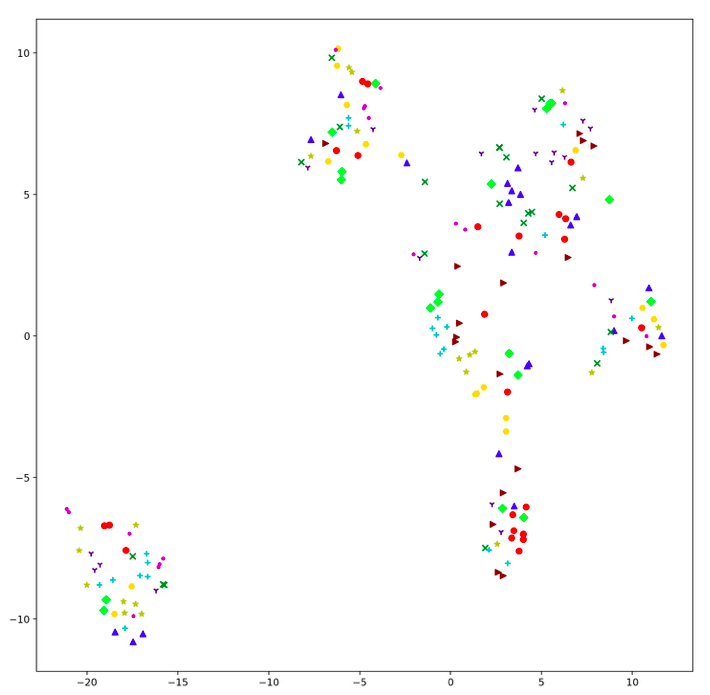
\includegraphics[width=0.5\textwidth]{images/Meanshift_Mall_4_6.png}
\end{center}
\caption{t-SNE projected result of Mean Shift with bandwidth = 0.2 on Mall Customers data set}
\label{fig:meanshift_mall_4_6}
\end{figure}

A more suitable clustering result is generated using a bandwidth of 27.5 (Figure \ref{fig:meanshift_mall_27}). In the plot, one can see that this value compensates between all four indexes.
When taking a look at the clustering result, there still are some data points which do not seem to be clustered correctly. One possible explanation concerns the gender column which is encoded as 0 and 1 (see section \ref{sec:mall_kmeans_evaluation}). It is not possible to calculate a meaningful distance between binary variables which may have an influence on the clustering result. 

\begin{figure}[H]
\begin{center}
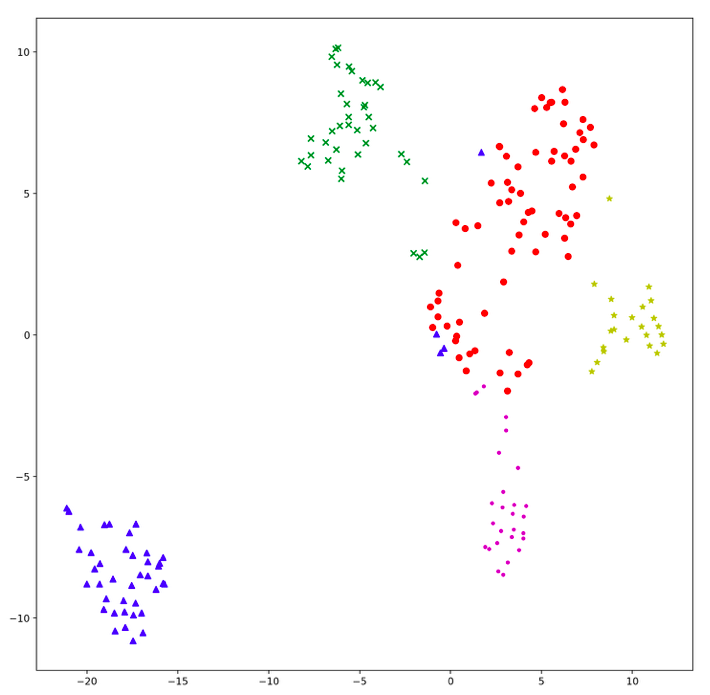
\includegraphics[width=0.5\textwidth]{images/Meanshift_Mall_27_5.png}
\caption{t-SNE projected result of Mean Shift with bandwidth = 27.5 on Mall Customers data set}
\label{fig:meanshift_mall_27}
\end{center}
\end{figure}

\subsubsection{Mall Customers - Affinity Propagation}
\textit{written by J.M.}\\

 \begin{figure}[H]
 	\begin{center}
 		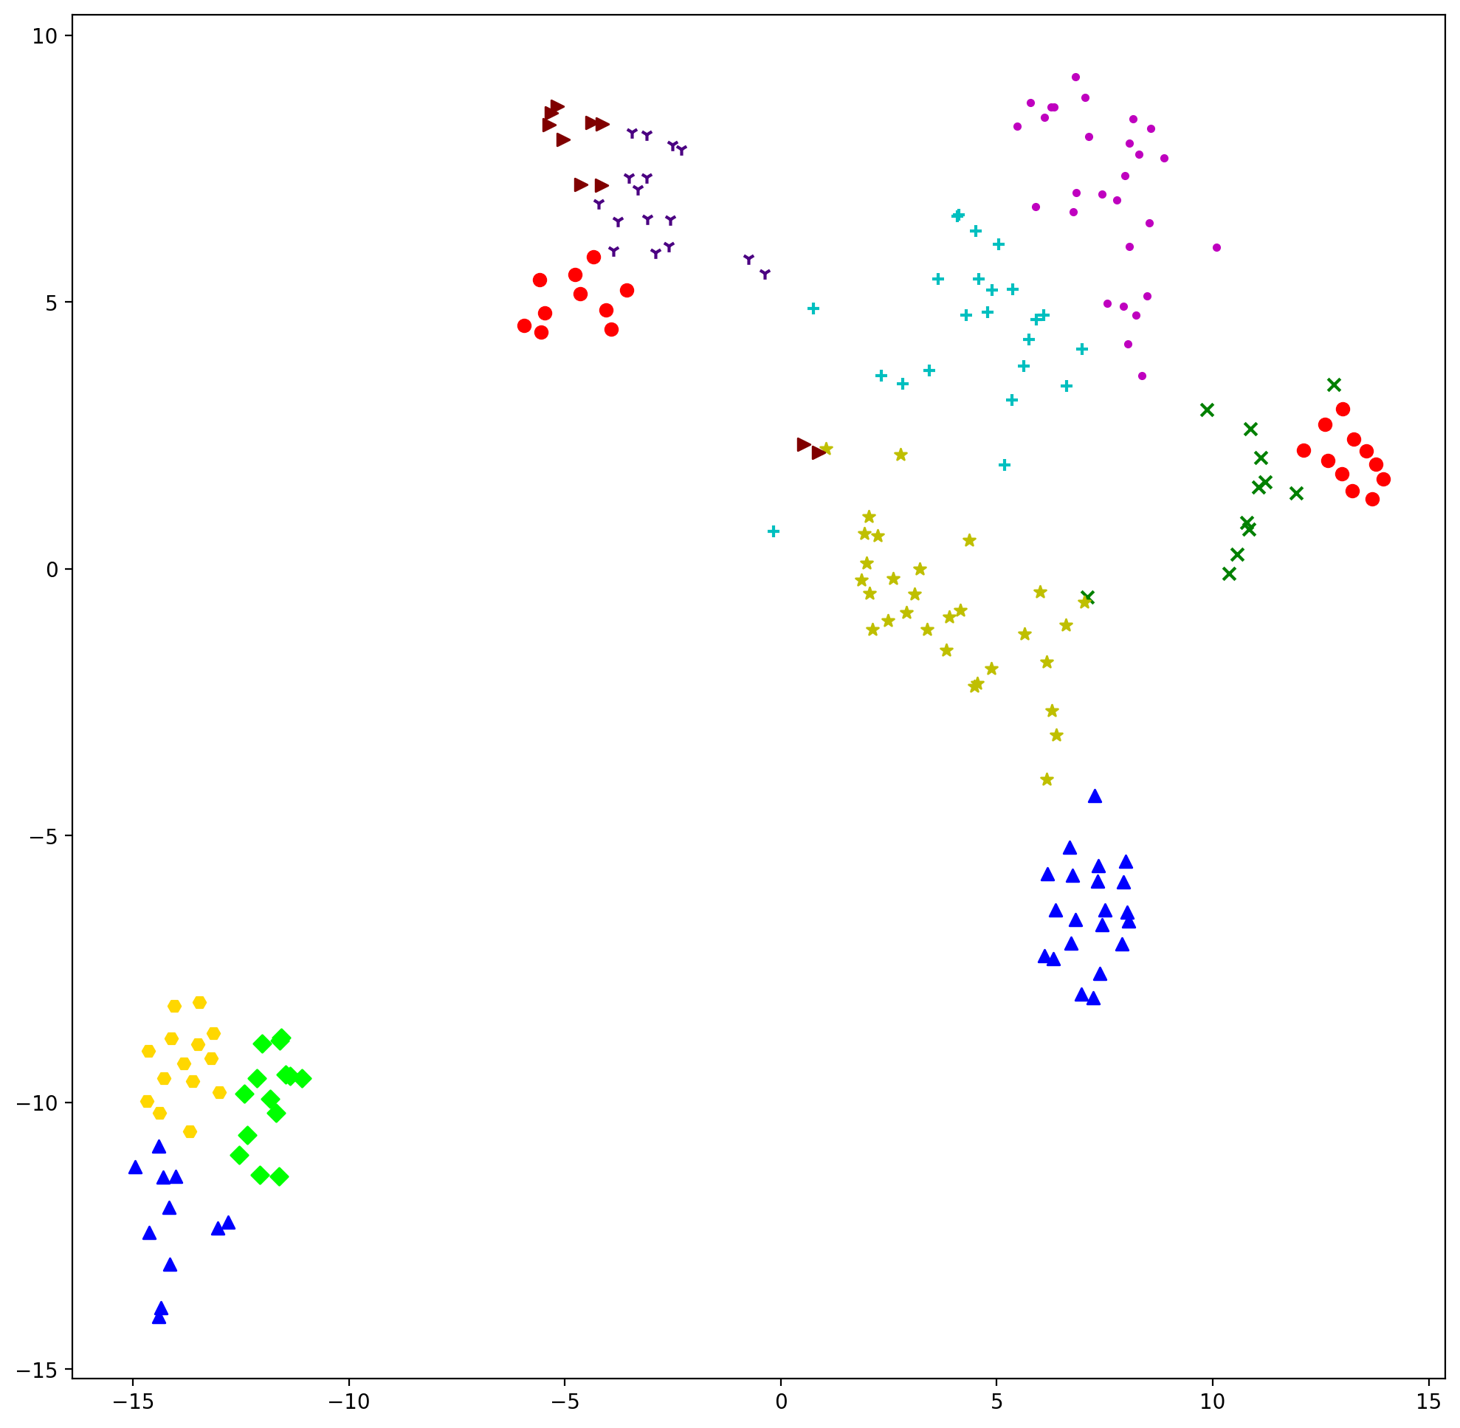
\includegraphics[width=0.5\textwidth]{images/af_mallcustomers2870.png}
 	\end{center}
 	\caption{t-SNE plot of Affinity Propagation on Mall Customers data set}
 	\label{fig:af_mall1}
 \end{figure}
 
 \begin{figure}[!ht]
 		\begin{center}
 			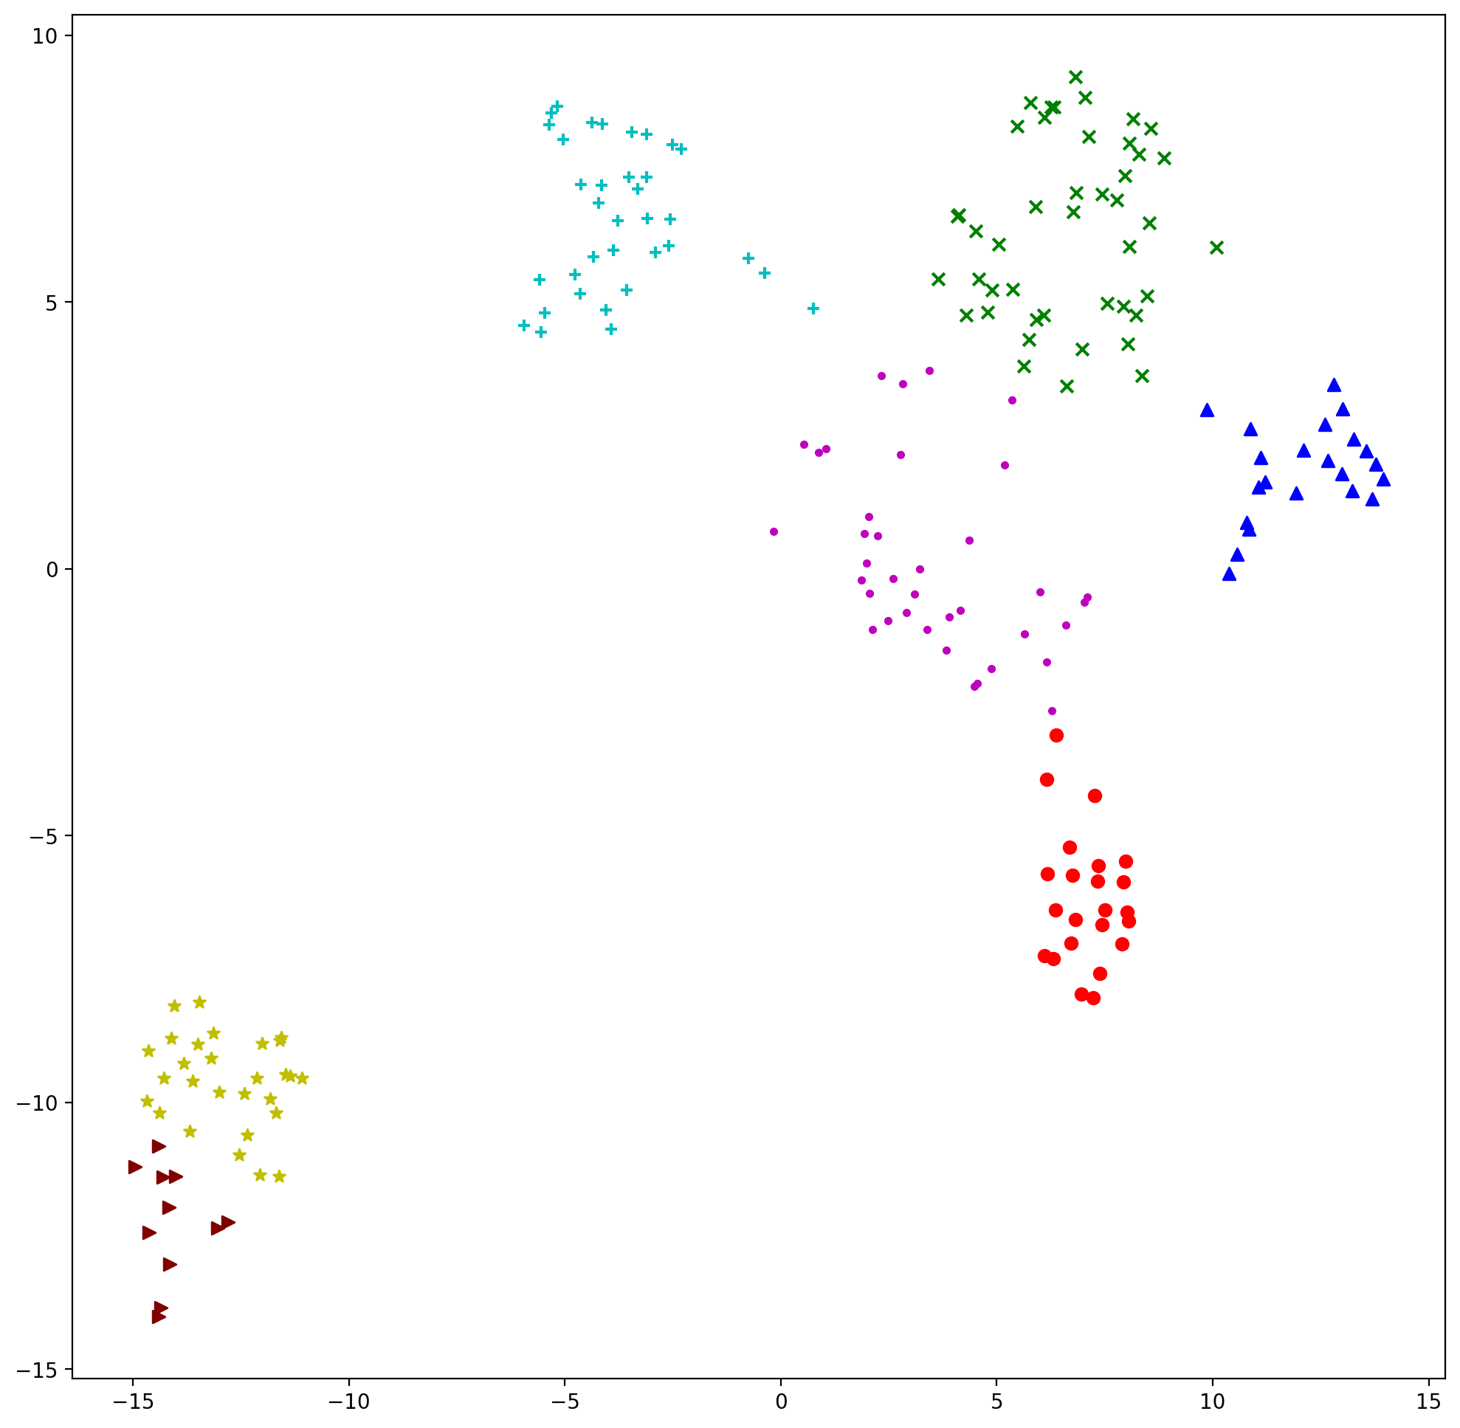
\includegraphics[width=0.5\textwidth]{images/af_mallcustomers8778.png}
 		\end{center}
 		\caption{t-SNE plot of Affinity Propagation on Mall Customers data set}
 		\label{fig:af_mall2}
 	\end{figure}
 
On the Mall Customers data set, Affinity Propagation also performs good, but for this data set the parameter is smaller as for the Seeds data set. In Figure \ref{fig:af_mall1} it computed with -2870. Here you see that the clustering is not good, there exist many clusters. To check if this algorithm works with this data set, the parameter is changed to a parameter value for which the clusters look good. This happened when the parameter is around -8778. This plot is in Figure \ref{fig:af_mall2}. If you compare these two plots with the cluster validation indexes, it confirms the obvious the Figure \ref{fig:af_mall2} is better. This parameter is also near to the optimum for this data set. 

\subsubsection{Mall Customers - Spectral Clustering}
\textit{written by M.A.}

\begin{figure}[H]
    \centering
    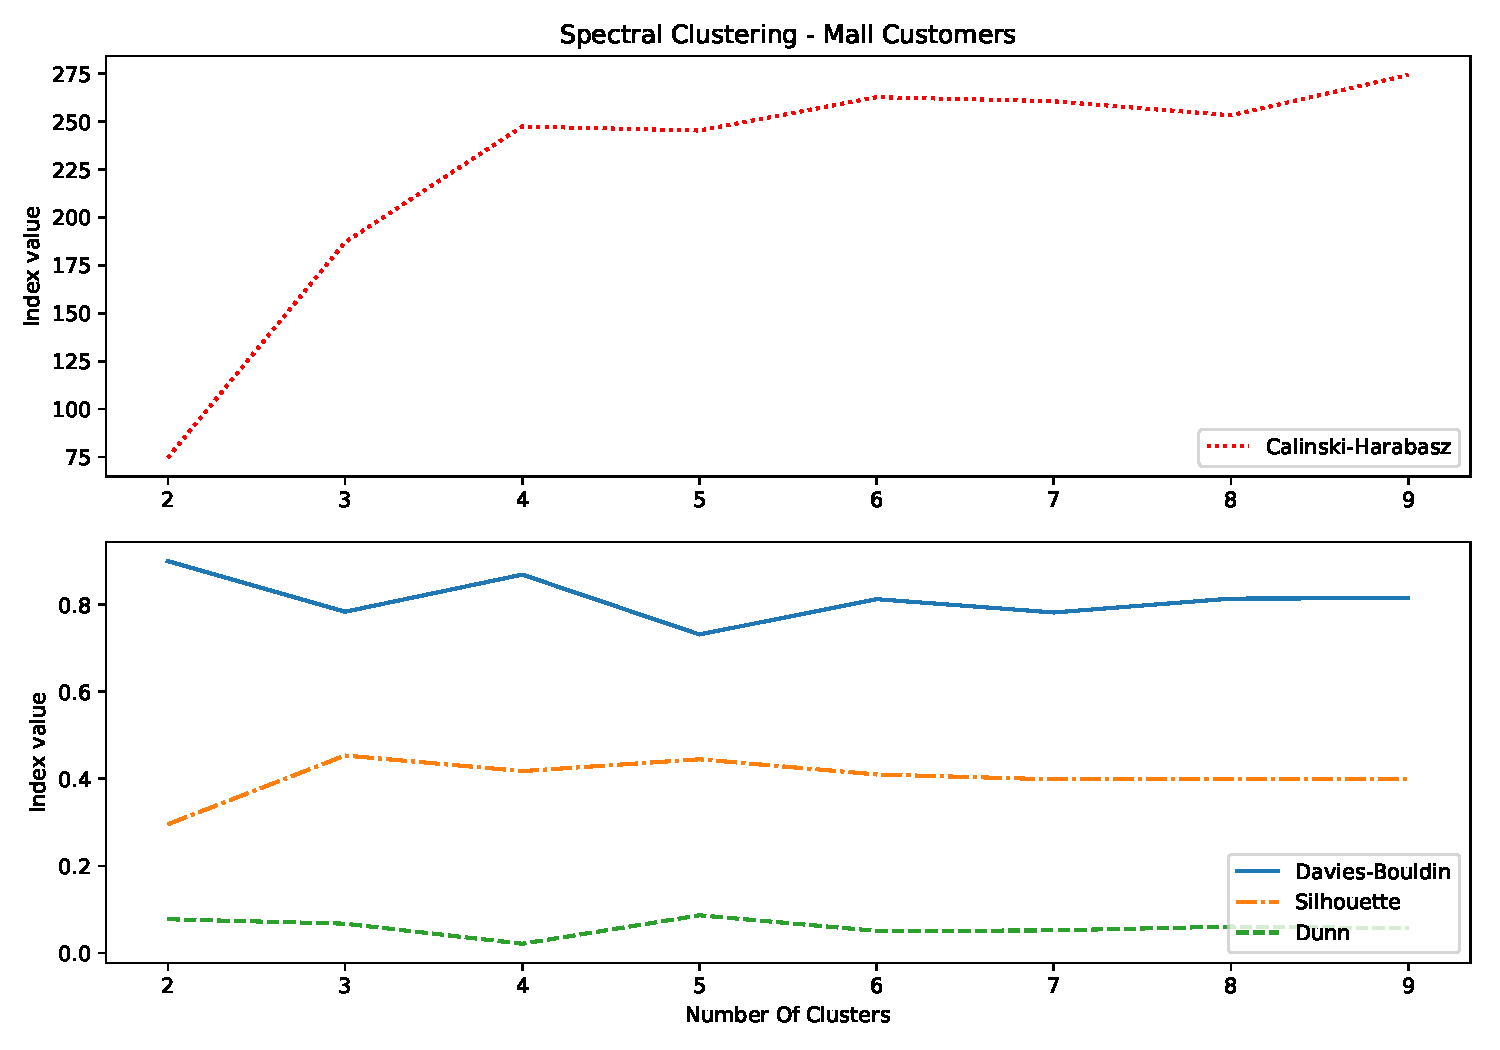
\includegraphics[width=1\textwidth]{images/Spectral_Clustering_-_Mall_Customers.pdf}
    \caption{Cluster validation indices by number of dimensions: Spectral Clustering on Mall Customers data set}
    \label{fig:my_label2}
\end{figure}

 
 Figure 23 depicts the influence of the \verb|n_cluster| parameter for the Spectral Clustering algorithm on the Mall data set. Analysing the line chart the same way as before, it can be determined that CH suggests 8 dimensions, whereas SI, DI and DB suggest 5 as the optimal dimensions. As the t-SNE projected result of Spectral Clustering is being plotted, it is being proved that Spectral Clustering is well applicable on the Mall Customers dataset, since it generates the plots very fast and easily. \newline
 
 
To decide which of these clusters is the optimal one, a plot for the dimension 5 and a plot for the dimension 8 is generated. Table 1 shows the plot1 with the dimension 5 and the plot 2 with the dimension 8. Comparing the cluster validation metrics of both plots, you can see that plot1 has better results regarding the maxima or rather minima (for DB). Even comparing to other parameters, there are not found better parameters than 5.\newline

\hspace{-0.75cm}
\resizebox{\textwidth}{!}{
\begin{tabular}{lrrrr}
 
 {}                            &  Calinski-Harabasz &  Davies-Bouldin &  Silhouette  &     Dunn \\ \hline 
 Plot 1  with the parameter 5  &     149.1555       &    0.8049       &     0.4461   &     0.0802  \\
 Plot 2   with the parameter 8 &     136.3805       &    1.0009       &     0.3510   &     0.0725 \\   \newline
 
 \end {tabular} 
} 
\begin{table}[H]
\caption{Comparison Cluster validation of Plot1 and Plot2 with Spectral Clustering}
\label{tab:evalutaion_table_spectral}
\end{table}
 %Table 1: Comparison Cluster validation of Plot1 and Plot2 with Spectral Clustering \newline
 
 \hspace{-0.25cm}
 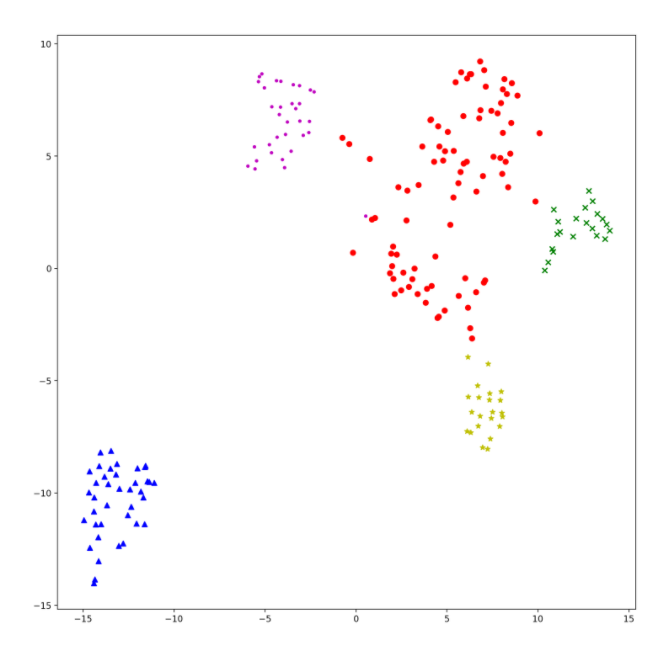
\includegraphics[width=0.5\textwidth]{images/5.PNG} 
 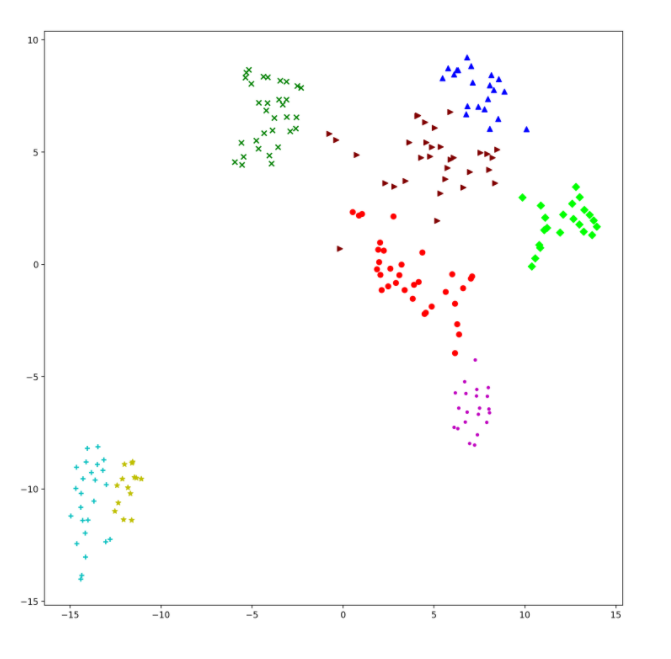
\includegraphics[width=0.5\textwidth]{images/8.PNG} 
 
 \begin{figure}[H]
    \centering
%     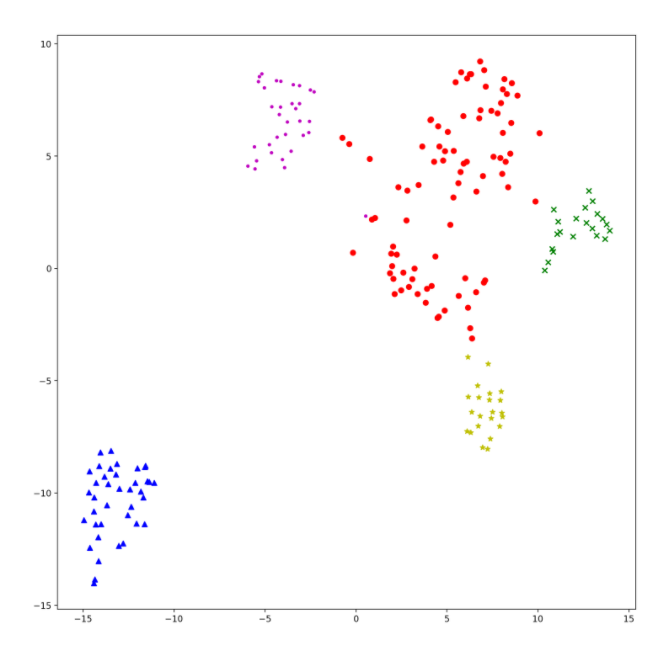
\includegraphics[width=0.5\textwidth]{images/5.PNG} 
 %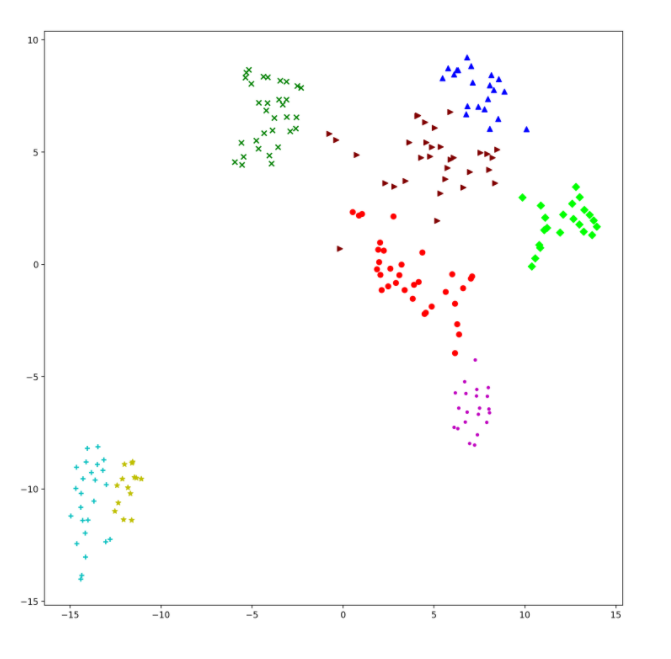
\includegraphics[width=0.5\textwidth]{images/8.PNG} 
    \caption{t-SNE projected result of Spectral Clustering with dimension = 5 (left) and dimension=9 (right)}
    \label{fig:my_label467}
\end{figure}
 %Figure 4:  t-SNE projected result of Spectral Clustering with dimension = 5 (left) and dimension=9 (right).
 
 



\subsubsection{House Pricing - K-Means}
\textit{written by B.L.}\\

This data set is challenging for K-Means clustering due to the high number of features. As described in section \ref{subsec:method_kmeans} the concept of distance does not hold up well in high dimensional cases. Attempts to transform the data into lower dimensional representations through principle component analysis did not yield an improvement in clustering performance. Data in Figure \ref{fig:kmeans_housing_indices_plot} suggests to consider 2 (\gls{DI}), 3 (\gls{SI}, \gls{DB}) or 4 (\gls{CH}) clusters.

\begin{figure}[H]
\begin{center}
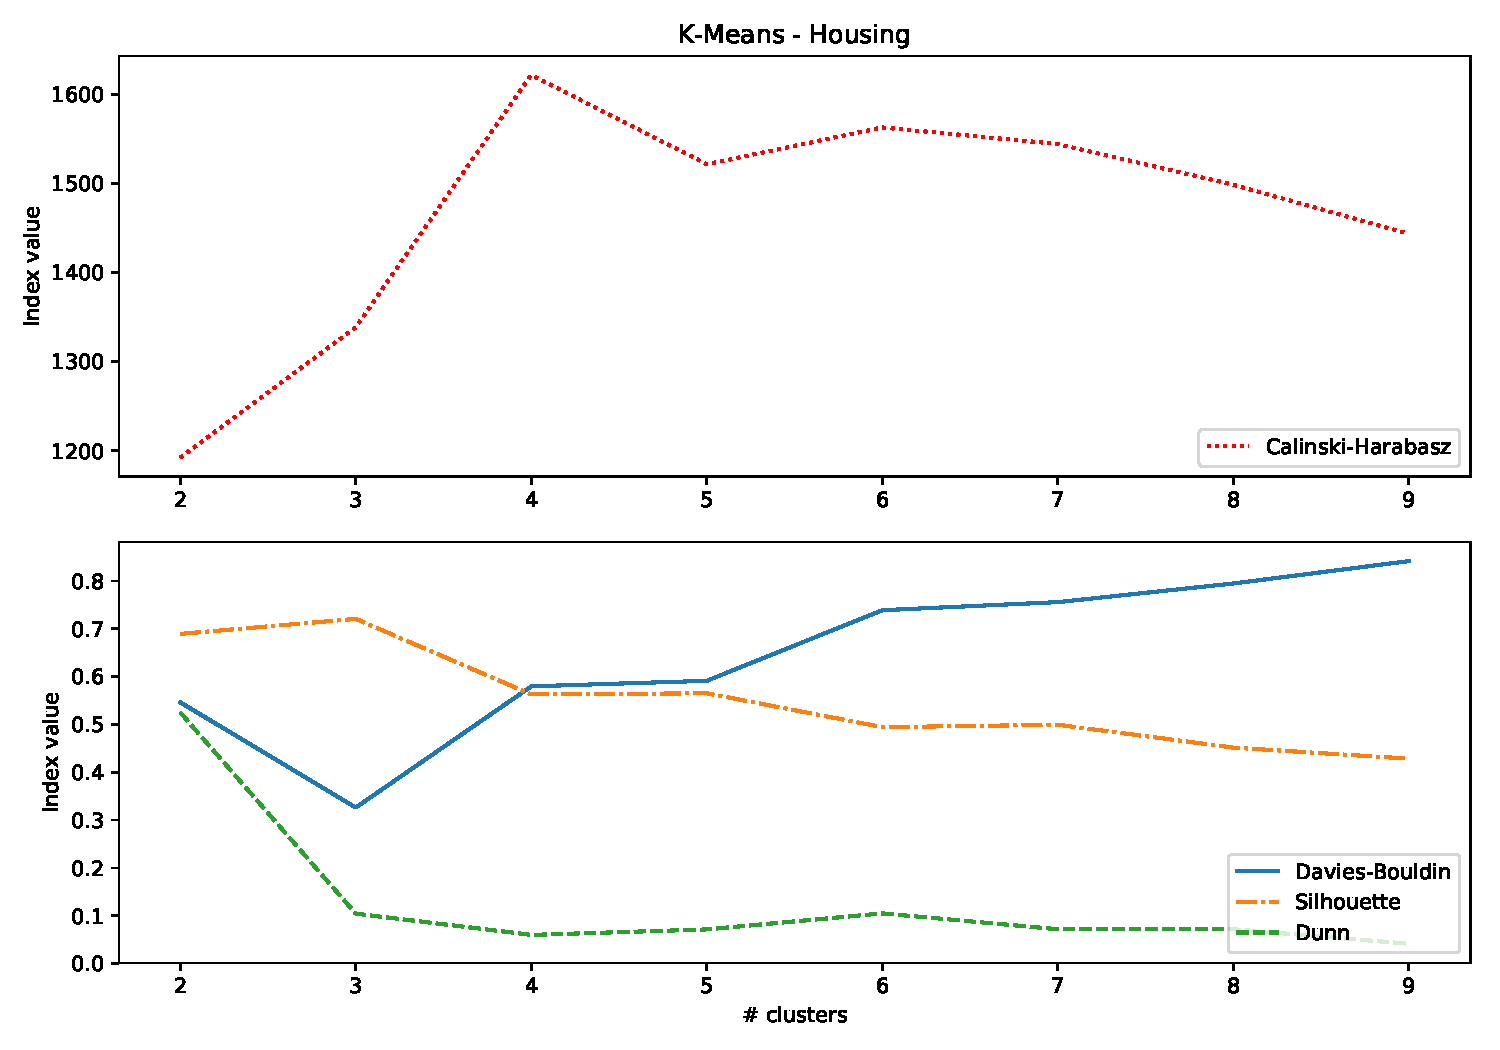
\includegraphics[width=1.0\textwidth]{images/kmeans_housing_index_plot.pdf}
\end{center}
\caption{K-Means Housing Data Set Indices by Number of Clusters}
\label{fig:kmeans_housing_indices_plot}
\end{figure}

Due to the high dimensionality of the data, looking at different angles in three dimensions to get an understanding is not feasible. Therefore a two dimensional transformation (t-SNE, see section \ref{sec:frontend_description}) will help. Figure \ref{fig:kmeans_housing_2d_comparison} shows the case of two, three and 15 as representation for a significantly higher number of clusters. From a visual standpoint, two and three clusters seem to capture the visibly separation of parts of the data quite well, while the high cluster count suggests it might be reasonable to consider the idea of there being a much more complex underlying structure to the data which is not well captured through the method at hand.

\begin{figure}[H]
\begin{center}
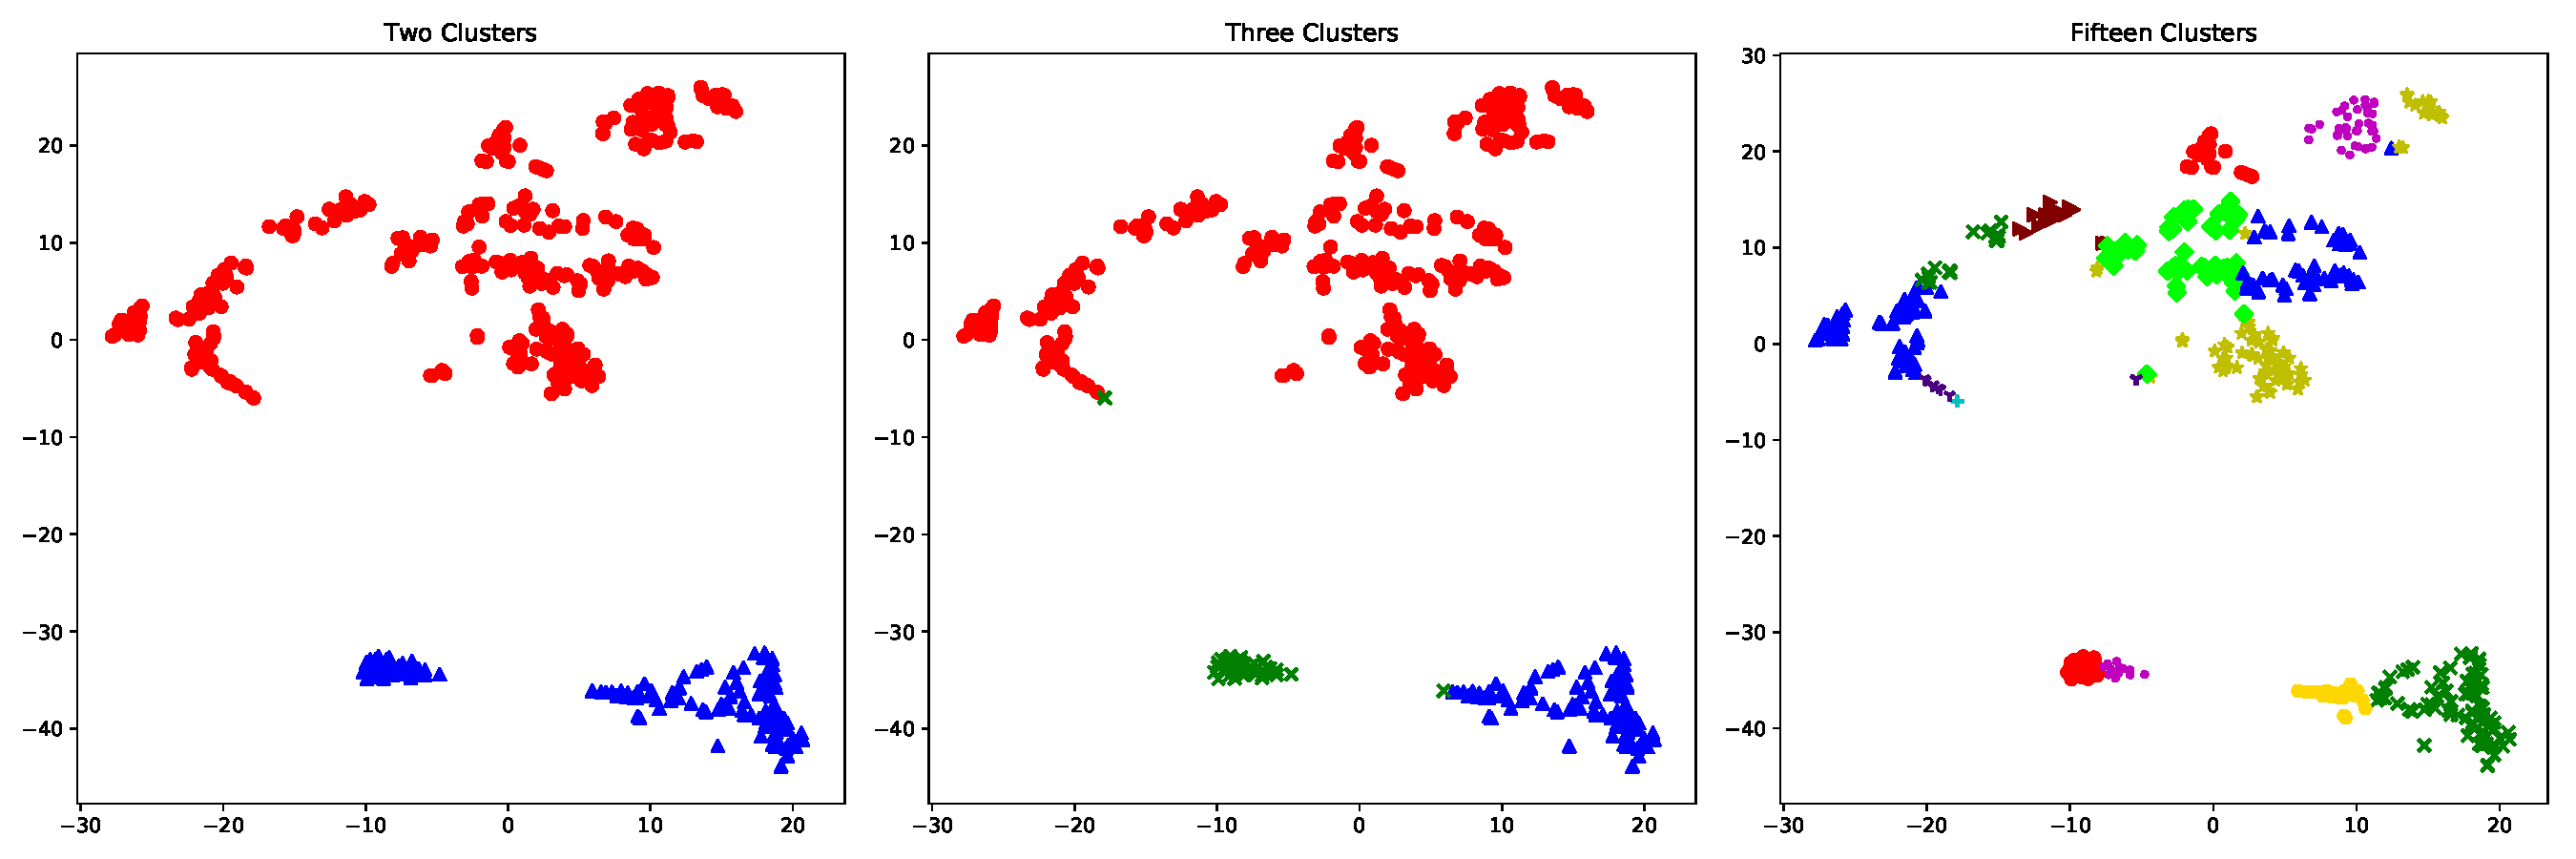
\includegraphics[width=1.0\textwidth]{images/kmeans_housing_tsne.pdf}
\end{center}
\caption{K-Means Housing Data Set t-SNE Transformed Data Plot}
\label{fig:kmeans_housing_2d_comparison}
\end{figure}
\vspace{-0.5cm}

\subsubsection{House Pricing - Mean Shift}
\textit{written by L.B.}\\

The third data set the Mean Shift algorithm was applied to is the Boston House Pricing data set. In contrast to the Seeds and the Mall Customers data set, it contains fourteen columns and hence requires the handling of fourteen dimensions. As mentioned in section \ref{sec:Mean Shift}, run time results in a complexity of $O(n^{3})$ in high dimensions. 
Nevertheless, Mean Shift seems to be able to handle the data set and produces reasonable clustering results. 

\begin{figure}[H]
\begin{center}
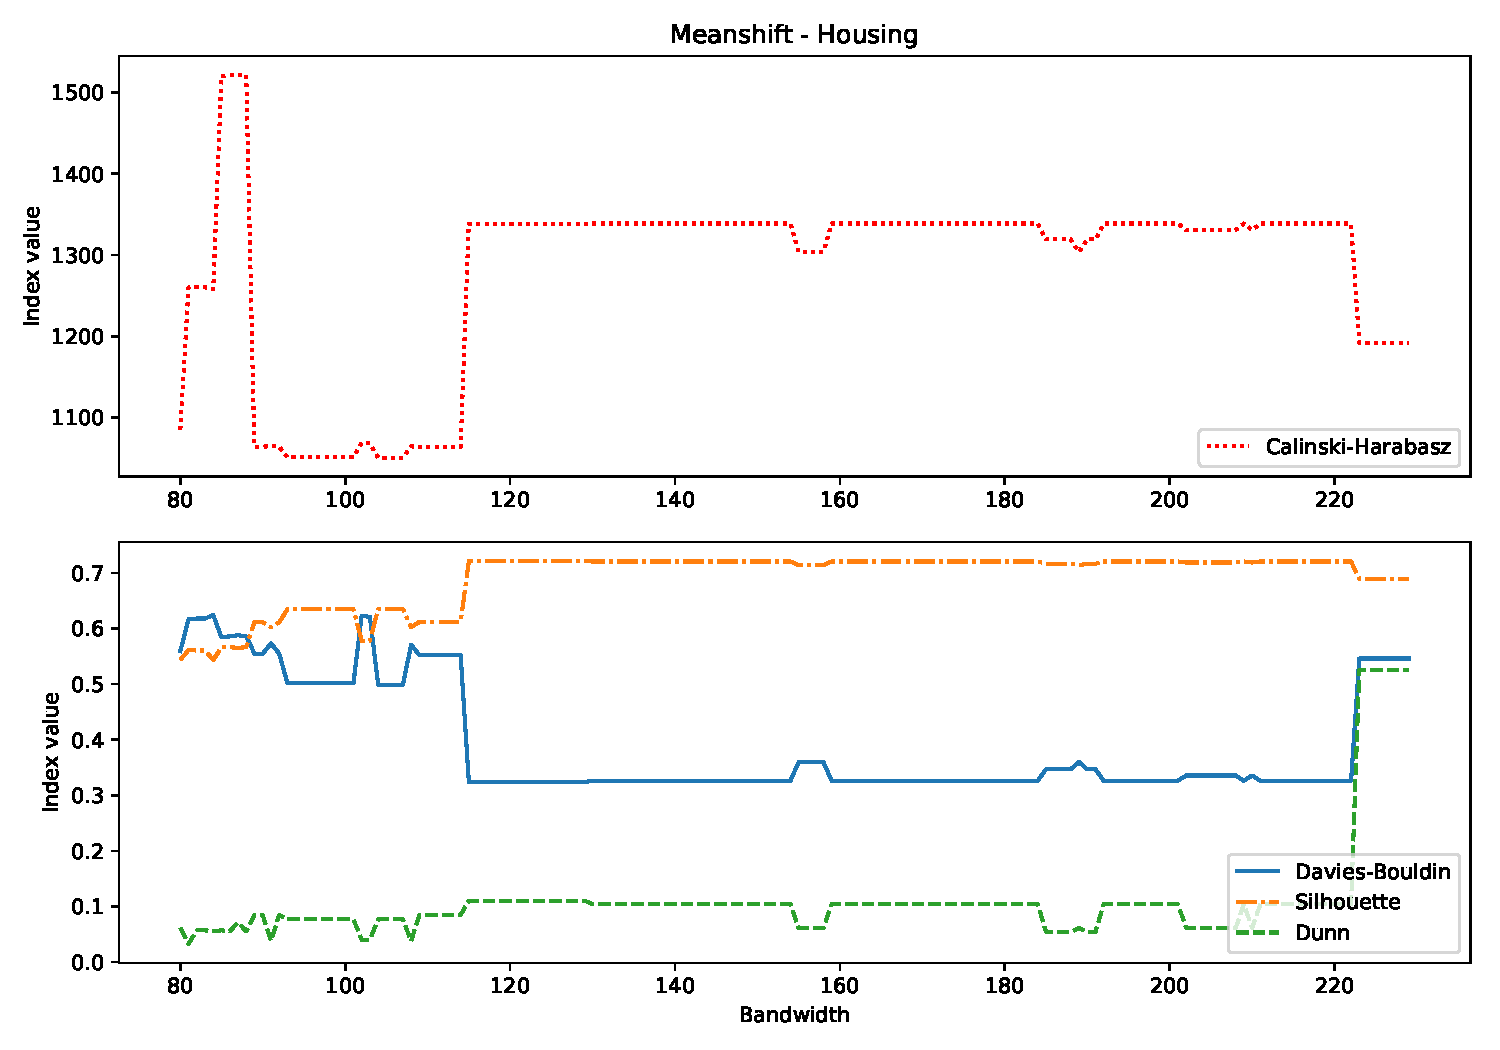
\includegraphics[width=0.8\textwidth]{images/Meanshift_-_Housing.pdf}
\end{center}
\caption{Cluster validation indexes: Mean Shift on House Pricing data set}
\label{fig:meanshift_housing_indexes}
\end{figure}

In Figure \ref{fig:meanshift_housing_indexes} one can clearly see a maximum of \gls{DI}, \gls{SI} and \gls{CH} and at the same time a minimum for \gls{DB} in the range of 118 to 156 or between 159 and 185. All of the four chosen cluster validation indexes do not change for either of the values within the mentioned ranges. This is due to the large distance between data points of the red cluster and the remaining data points as it can be seen in Figure \ref{fig:meanshift_housing_120}.

\begin{figure}[H]
\begin{center}
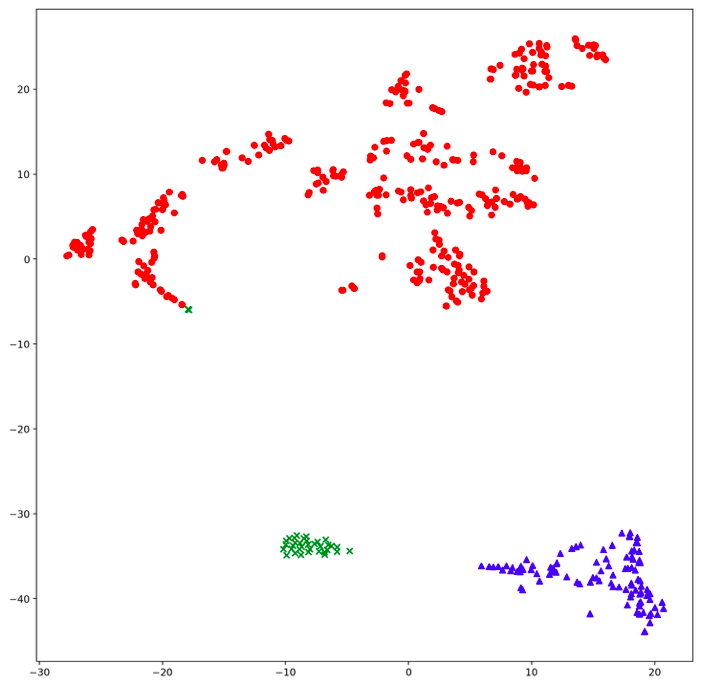
\includegraphics[width=0.5\textwidth]{images/Meanshift_Housing_120.png}
\end{center}
\caption{t-SNE projected result of Mean Shift with bandwidth = 120 on House Pricing data set}
\label{fig:meanshift_housing_120}
\end{figure}

The bandwidth value determines the kernel's radius and thus influences which data points are considered for which cluster. If data points are far away from each other, as it is the case for the Boston House Pricing data set, increasing the bandwidth parameter will not include any more data points within the kernel's radius and thus not have an influence on the cluster generation. 

Furthermore, the data set consists of three relatively dense regions far away from each other, which is a desirable situation when applying density-based clustering algorithms. Due to this, Mean Shift algorithm performs well on the data set, even though it is high-dimensional.

\subsubsection{House Pricing - Affinity Propagation}
\textit{written by J.M.}\\

On the House Pricing data set, Affinity Propagation performs not good. It takes some time to find a good parameter for this data set. This is shown in Figure \ref{fig:af_house1}. The parameter for this plot was -71433. This parameter is so low because this data set has the most dimensions. If you use a higher parameter, the cluster is not so good. This is shown in Figure \ref{fig:afhouse2}.   

\begin{figure}[H]
		\begin{center}
			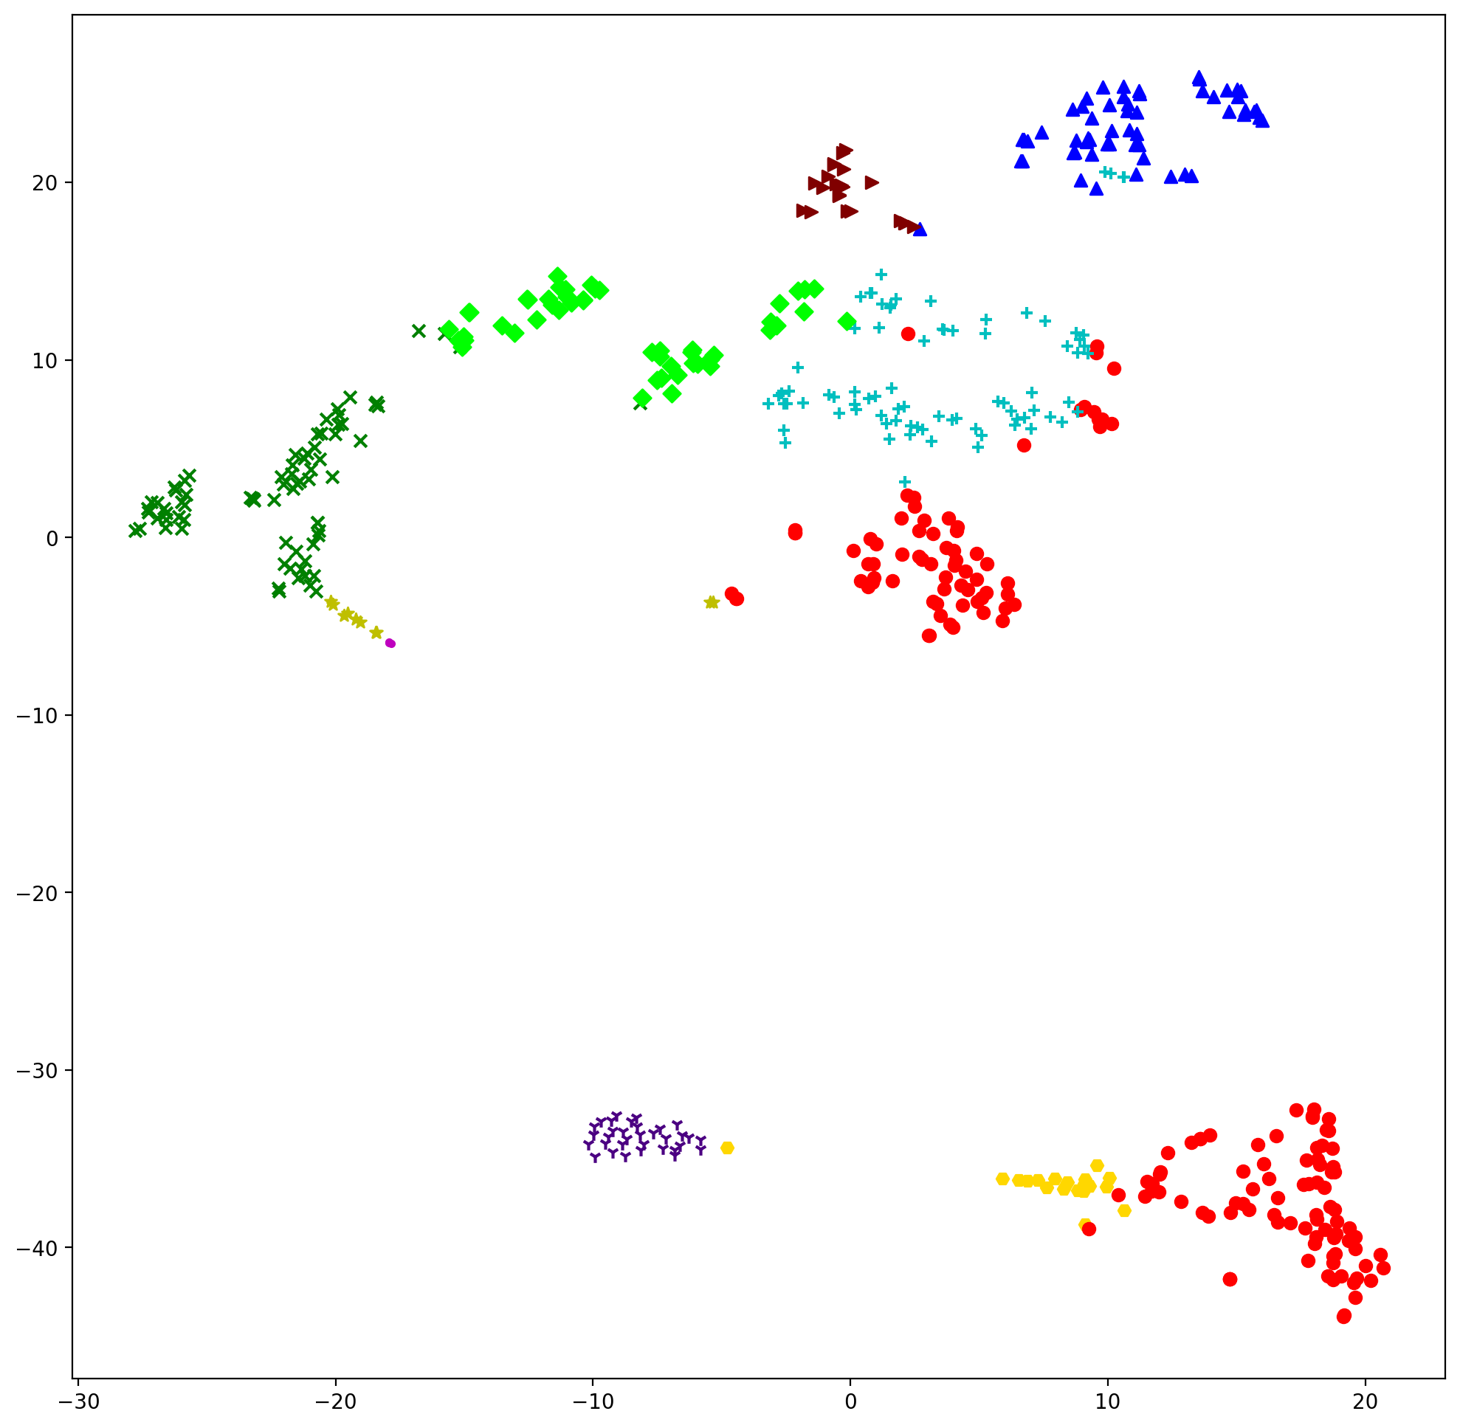
\includegraphics[width=0.5\textwidth]{images/af_housepricing71433.png}
		\end{center}
		\caption{t-SNE plot of Affinity Propagation on House Pricing data set}
		\label{fig:af_house1}
	\end{figure}
	
	\begin{figure}[H]
			\begin{center}
				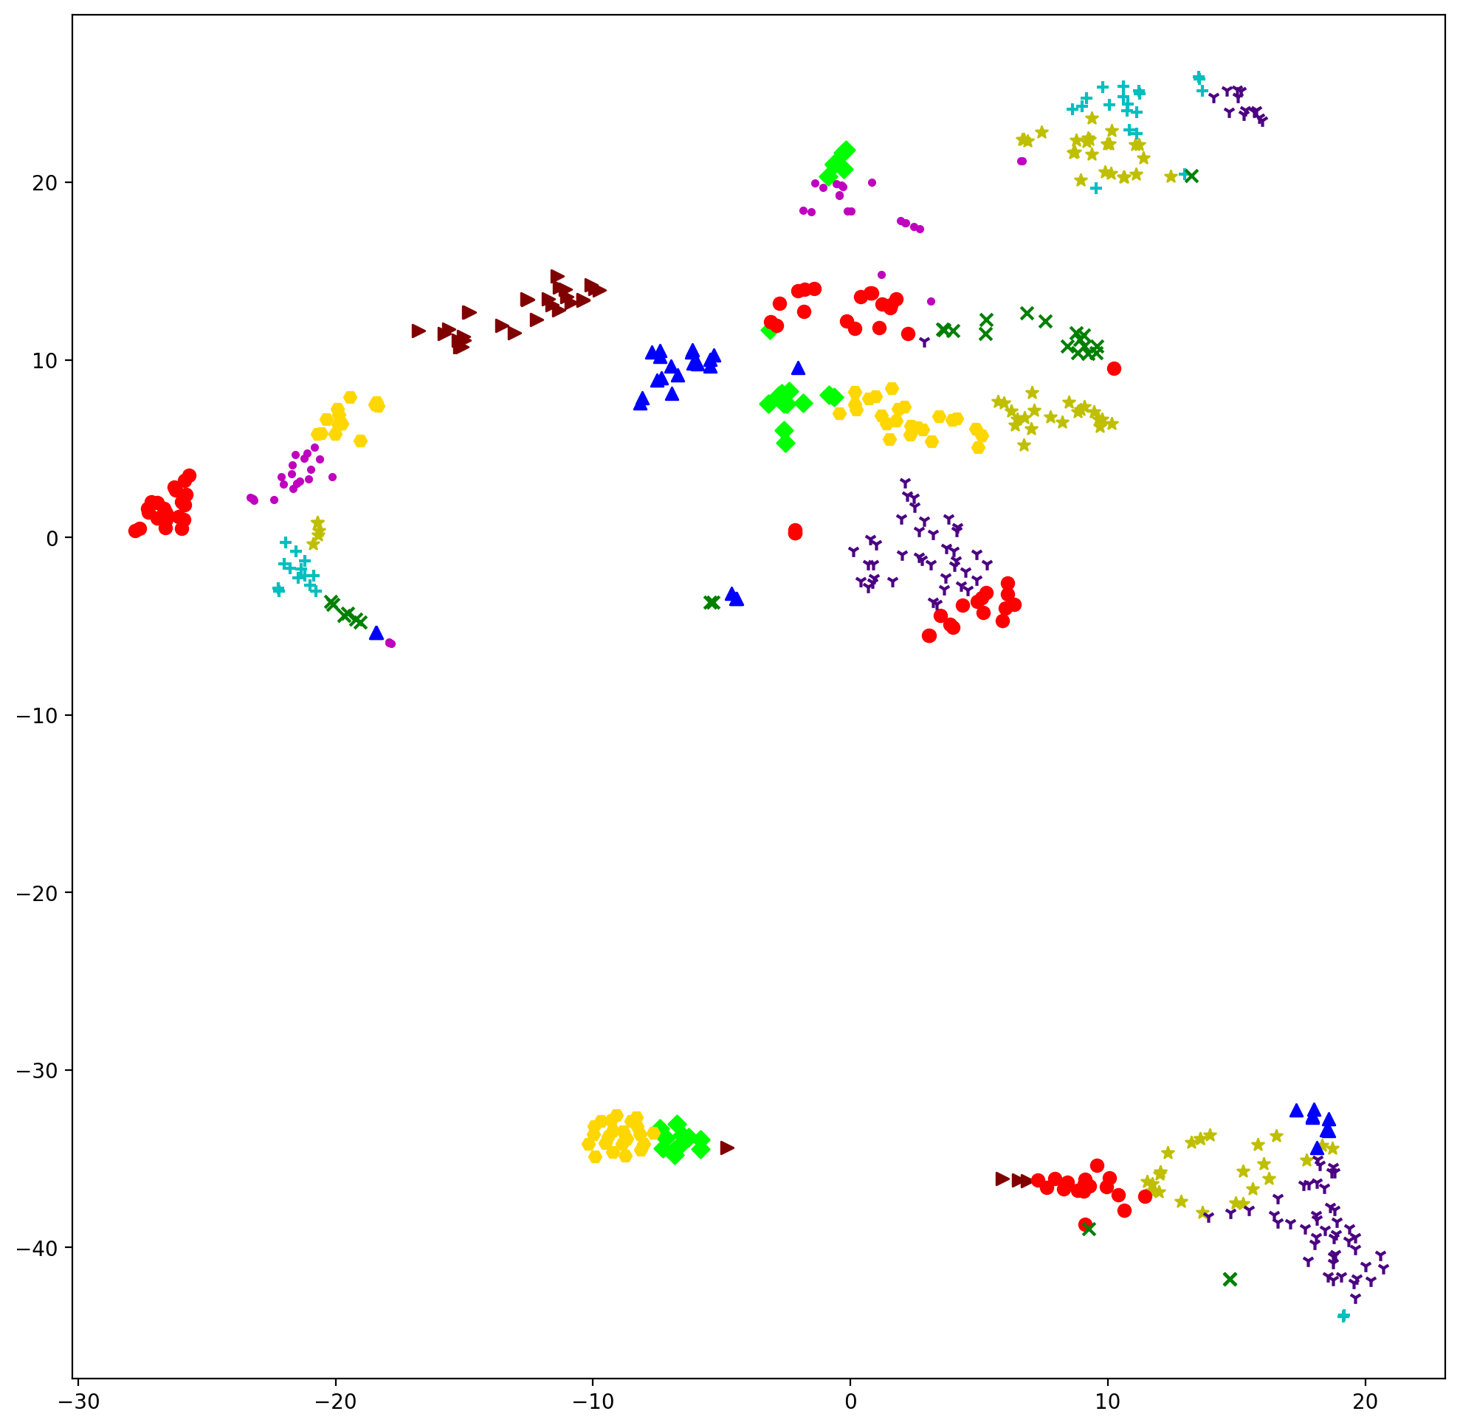
\includegraphics[width=0.5\textwidth]{images/af_housepricing6900.png}
			\end{center}
			\caption{t-SNE plot of Affinity Propagation on House Pricing data set}
			\label{fig:afhouse2}
		\end{figure}

\subsubsection{House Pricing - Spectral Clustering}
\textit{written by M.A.}\\

The following Cluster validation indices how Spectral Clustering performed on the House Pricing data set. \newline
 
  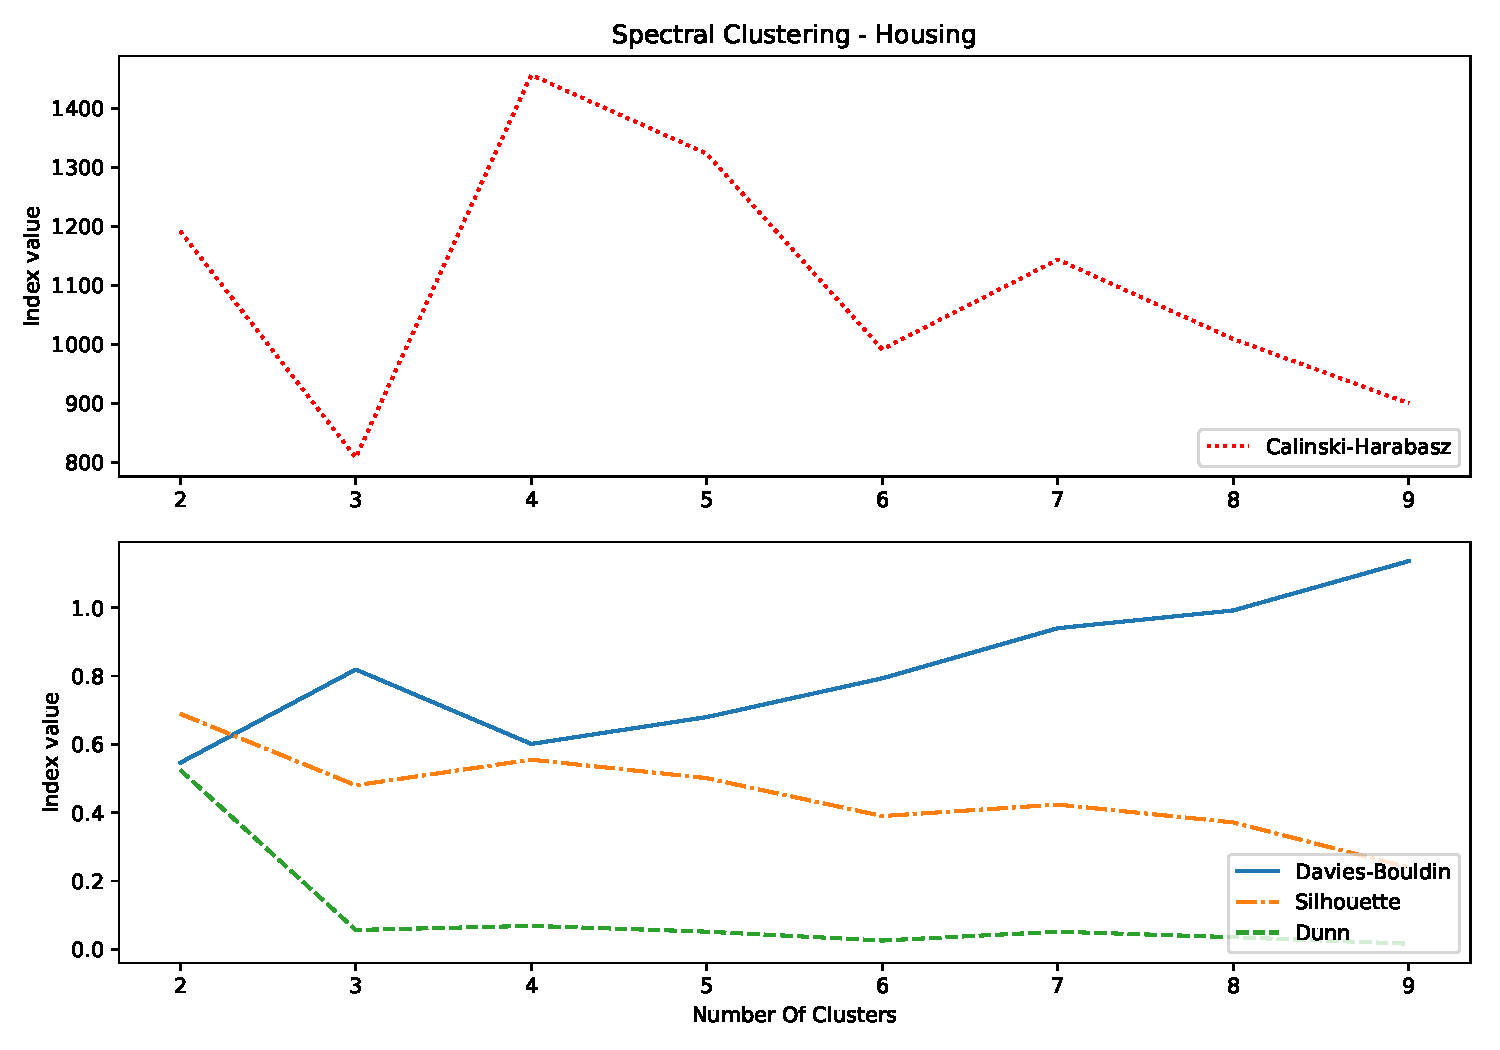
\includegraphics[width=1\textwidth]{images/Spectral_Clustering_-_Housing.pdf} \newline
 Figure 5: Cluster validation indices by number of dimensions: Spectral Clustering on House Pricing data set.\newline
 
 On the House Pricing data set, Spectral Clustering works good as well. The calculation to build the clusters is very fast. Figure depicts the plots of the clustering with the dimension 2,4 and 6. \newline
 
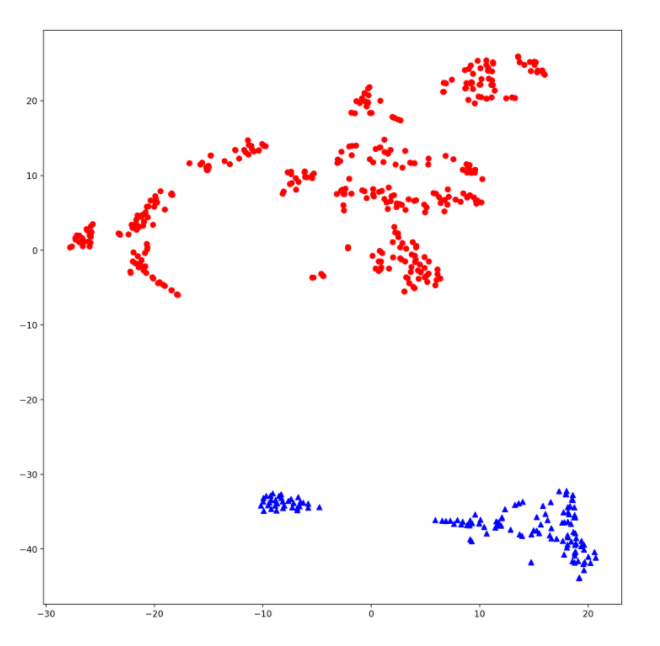
\includegraphics[width=0.3\textwidth]{images/2.PNG} 
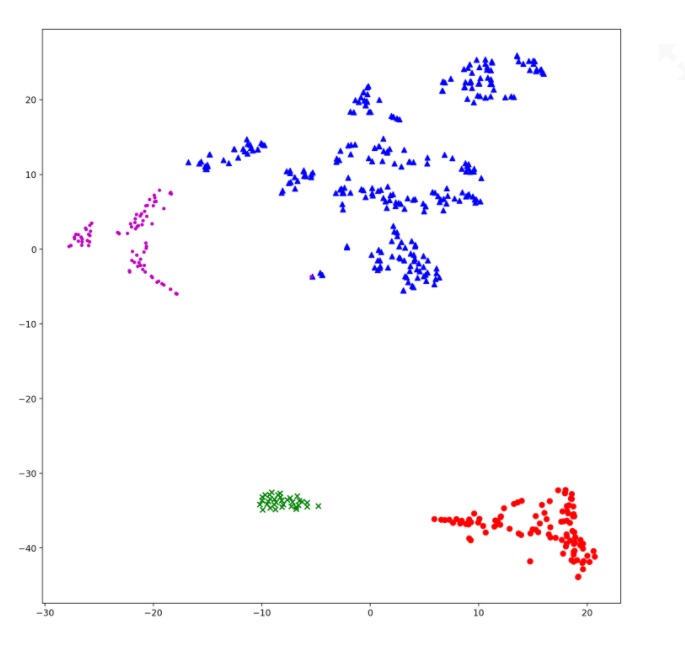
\includegraphics[width=0.3\textwidth]{images/4.PNG} 
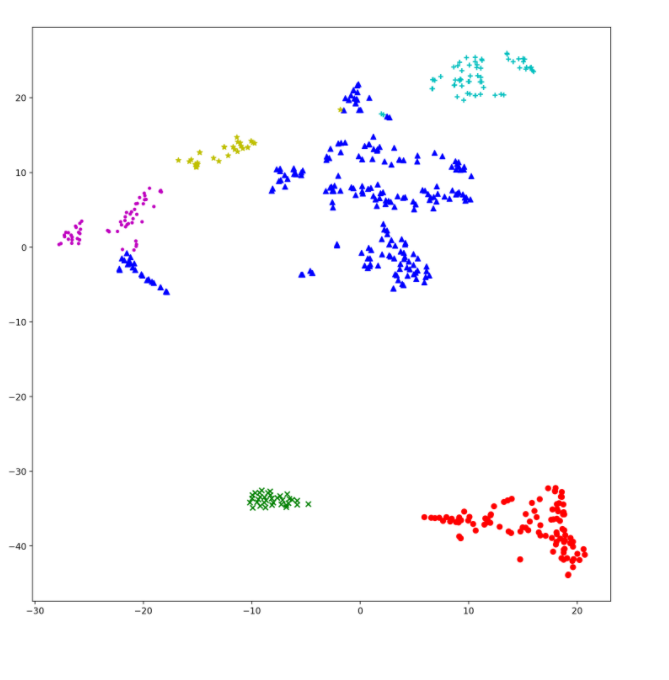
\includegraphics[width=0.3\textwidth]{images/6.PNG} \newline
  
 Figure 32:  t-SNE projected result of Spectral Clustering with dimension 2,4 and 6 (from left to right). \newline

\subsubsection{Wine Quality - K-Means}
\textit{written by B.L.}\\


The wine data set again presents a challenge due to its high feature count as well as having one discrete feature. Dimensionality reduction helps to speed up calculation but does not show an improvement in evaluation index performance. The plot of evaluation indices in Figure \ref{fig:kmeans_wine_indices_comparison} gives an indication for 2 (\gls{SI}, \gls{DB}), 3 (\gls{CH}), or 6 (\gls{CH}, \gls{DB}) clusters

\begin{figure}[H]
\begin{center}
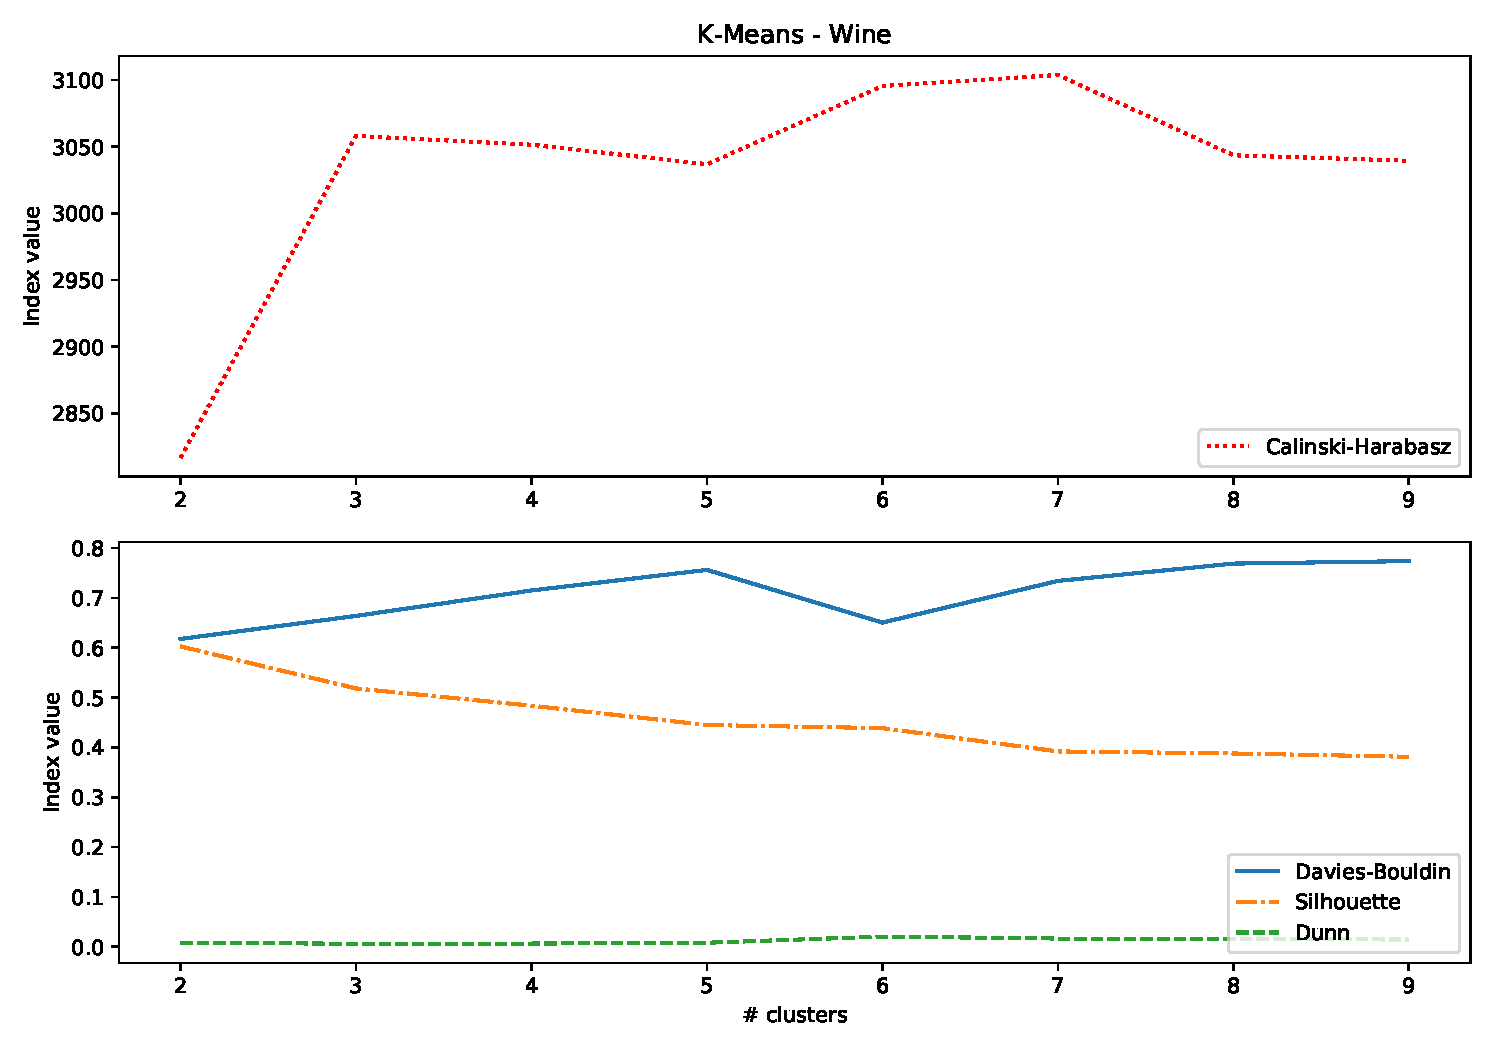
\includegraphics[width=1.0\textwidth]{images/kmeans_wine_index_plot.pdf}
\end{center}
\caption{K-Means Wine Data Set Indices by Number of Clusters}
\label{fig:kmeans_wine_indices_comparison}
\end{figure}

but looking at the two dimensional transformed data in Figure \ref{fig:kmeans_wine_tsne} for three and six clusters compared to the original labeling does not allow for any interpretation due to the fact that little about structure - if it exists - can be learned from the original labels.

%does not allow for any visual evaluation concerning the quality of fit.

%The result is inconclusive and without a focus on feature engineering other methods may be better suited to deal with this data set.


\begin{figure}[H]
\begin{center}
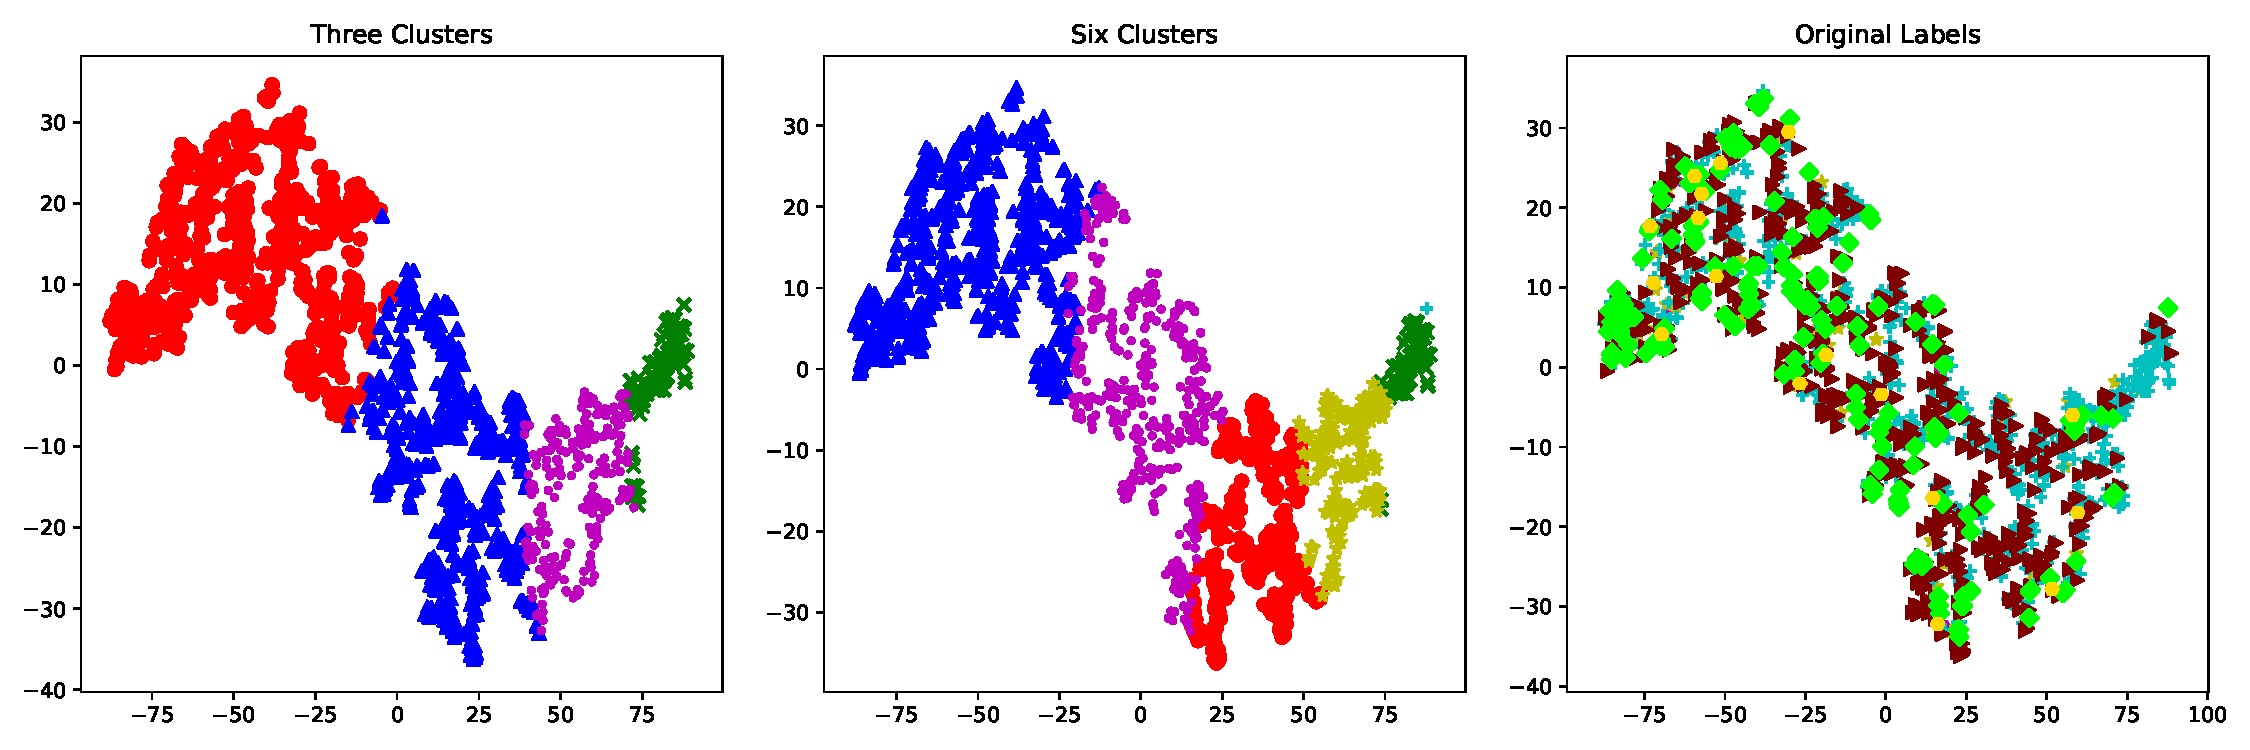
\includegraphics[width=1.0\textwidth]{images/kmeans_wine_tsne.pdf}
\end{center}
\caption{K-Means Wine Data Set Indices by Number of Clusters}
\label{fig:kmeans_wine_tsne}
\end{figure}

Looking back at the PCA step mentioned before, the picture becomes clearer when utilizing it as a visualization support and looking at a three dimensional representation of the transformed data in Figure \ref{fig:kmeans_wine_3d_multi} gives a clearer understanding of how the clustering has worked out. The component driving the differentiation between clusters called \textit{PCA 1} captures 94\% of the variance and loadings show it being driven in large part by the two \textit{sulfur} concentration features.

\begin{figure}[H]
\centering
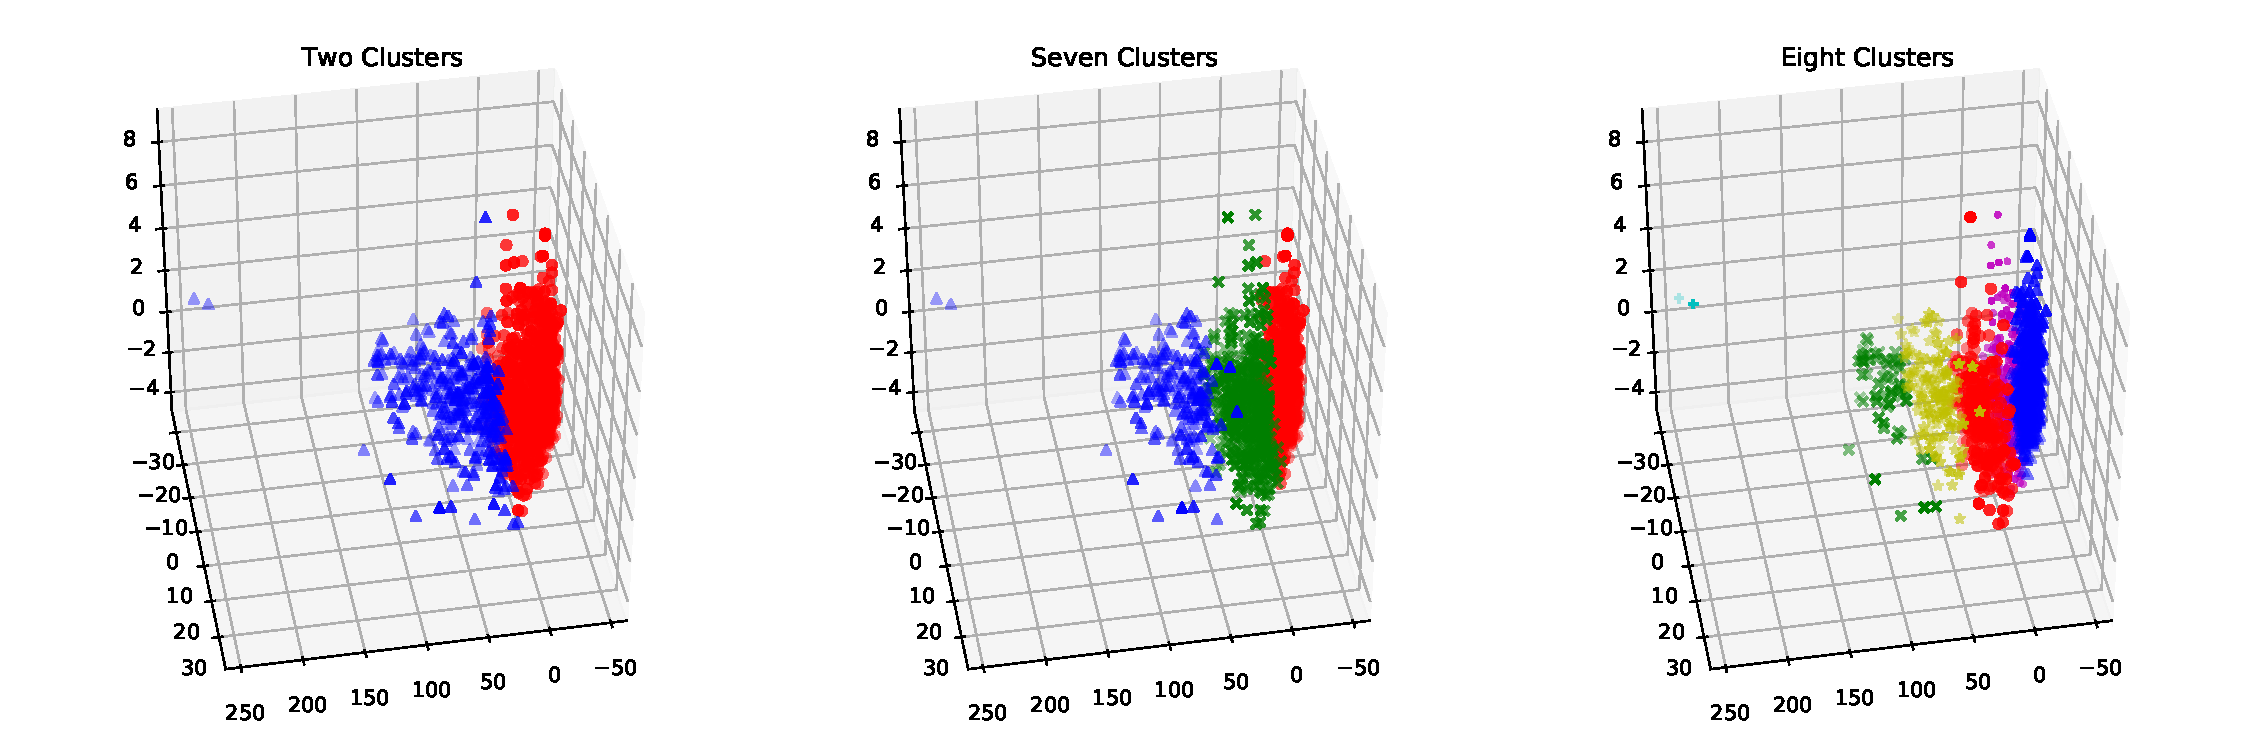
\includegraphics[width=1.0\textwidth]{images/kmeans_wine_3d_multi.pdf}
\caption{Wine Data Set 3D Plot Clustering Options}
\label{fig:kmeans_wine_3d_multi}
\end{figure}

\newpage
\vspace{-0.5cm}
\begin{wrapfigure}{r}{0.5\textwidth}
  \centering
    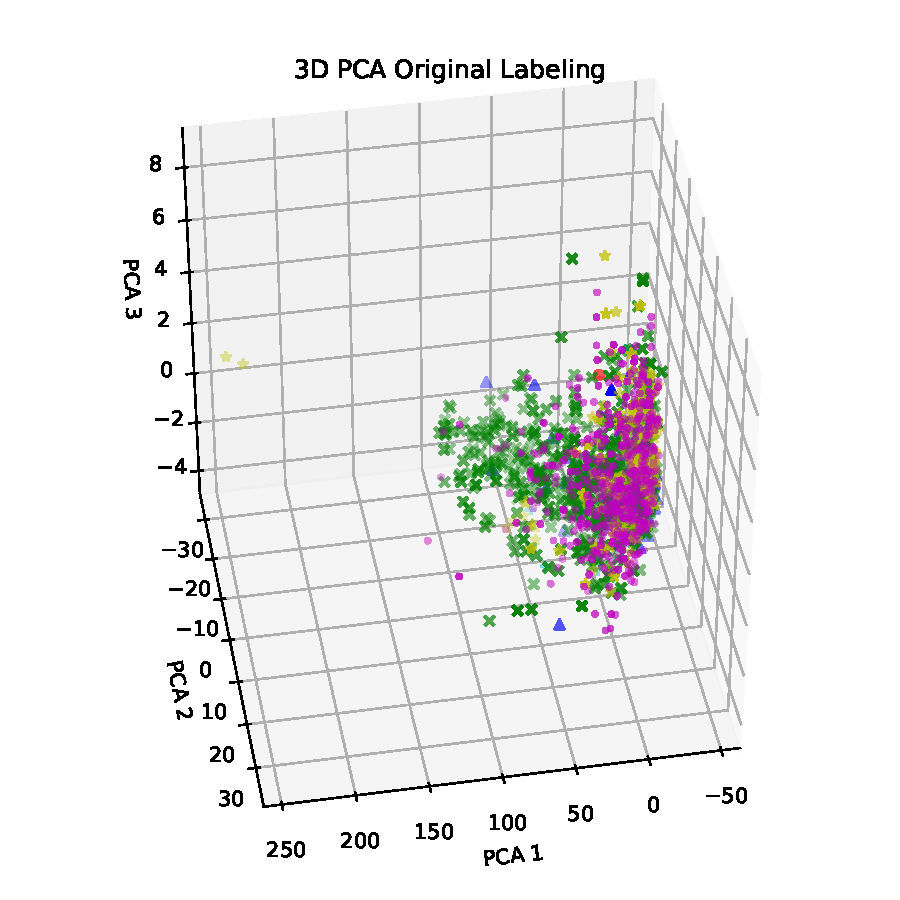
\includegraphics[trim={1cm 0cm 1cm 1cm},width=0.45\textwidth, clip]{images/kmeans_wine_pca_original.pdf}
  \caption{Wine 3D Original Labeling}
  \label{fig:kmeans_wine_pca_original}
\end{wrapfigure}

Looking at the original labeling of the data however shows the limitations of clustering and especially K-Means clustering for this data set. Figure \ref{fig:kmeans_wine_pca_original} shows the same projection as Figure \ref{fig:kmeans_wine_3d_multi} but this time with the original labeling. The math on accuracy and recall at 19.8\% and precision somewhat better at 58.2\% also shows the less than optimal performance. However this is not unexpected when considering the strengths and weaknesses of K-Means described in section \ref{subsec:method_kmeans}: contiguous, non-overlapping, convex clusters can be captured well while at least this representation of the data displays a lack of these characteristics in the data set.


\subsubsection{Wine Quality - Mean Shift}
\textit{written by L.B.}\\

Applying Mean Shift algorithm to the last data set shows that density-based clustering is also able to identify non-convex clusters. The following plots demonstrate how Mean Shift clustering performed on the Red Wine Quality data set along different values for the required bandwidth parameter.

\begin{figure}[H]
\begin{center}
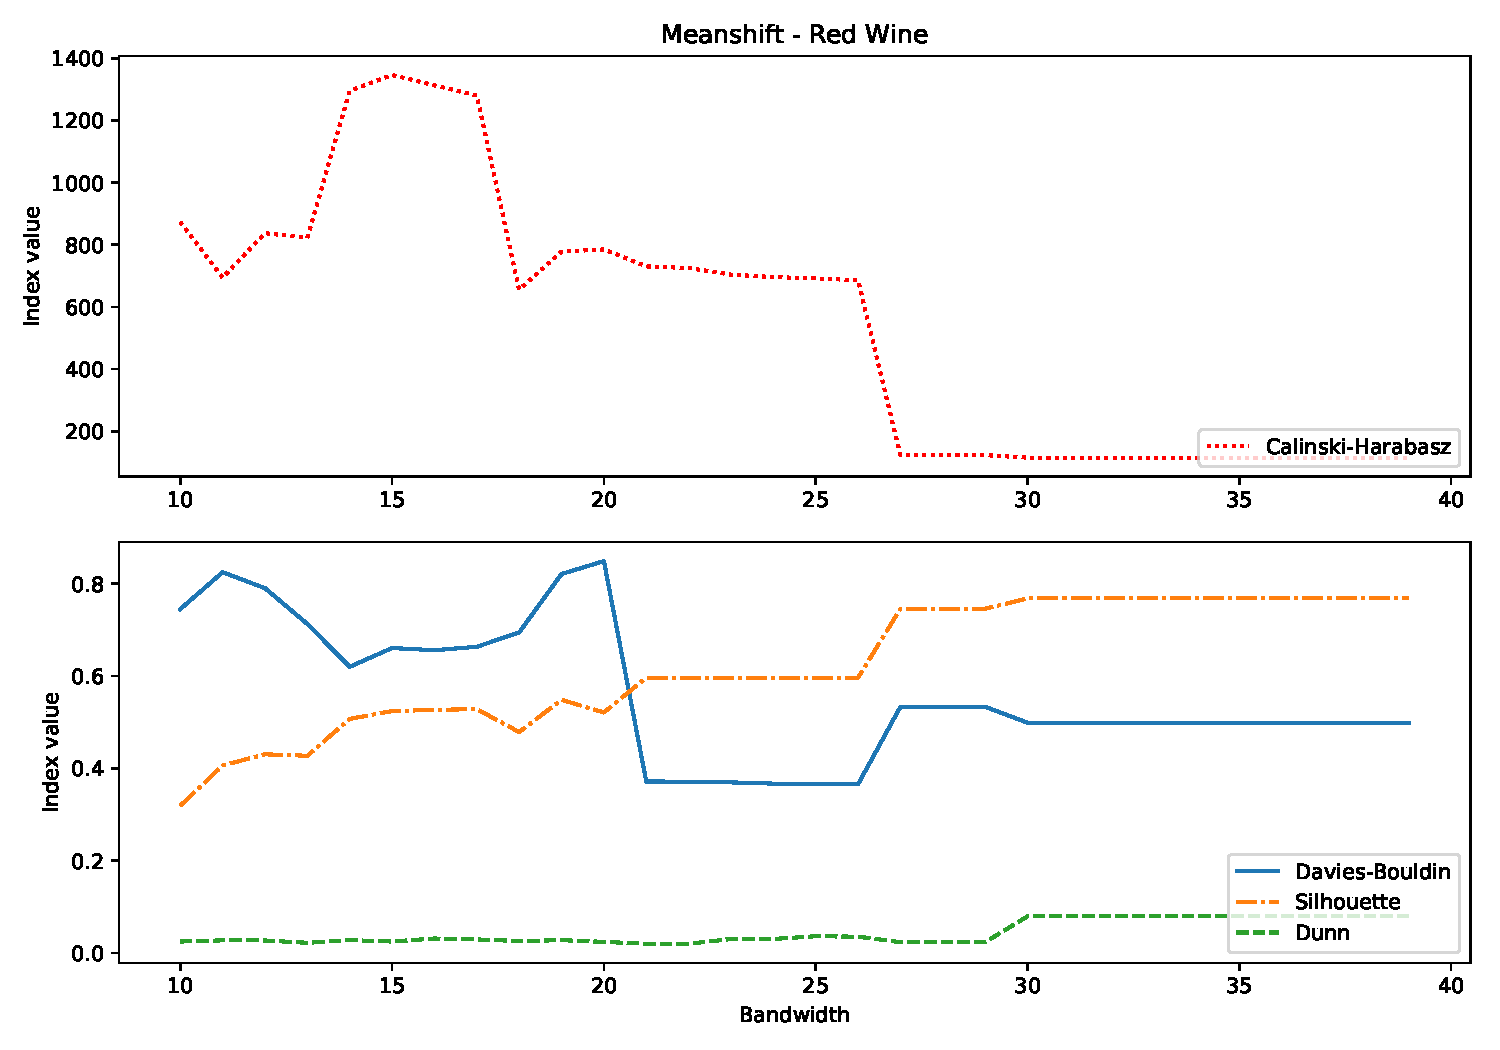
\includegraphics[width=0.8\textwidth]{images/Meanshift_-_Red_Wine.pdf}
\end{center}
\caption{Cluster validation indexes: Mean Shift on Red Wine Quality}
\label{fig:meanshift_wine_indexes}
\end{figure}

The cluster validation indexes suggest that a bandwidth parameter of 22.5 generates the best clustering results. However, the overall performance on this data set is worse compared to the House Pricing data set, even though consists of less dimensions. This is the case as data points of the Wine Quality data set lie relatively close together and no distant and clearly separated dense regions can be identified (Figure \ref{fig:meanshift_wine_22_5}). 

\begin{figure}[H]
\begin{center}
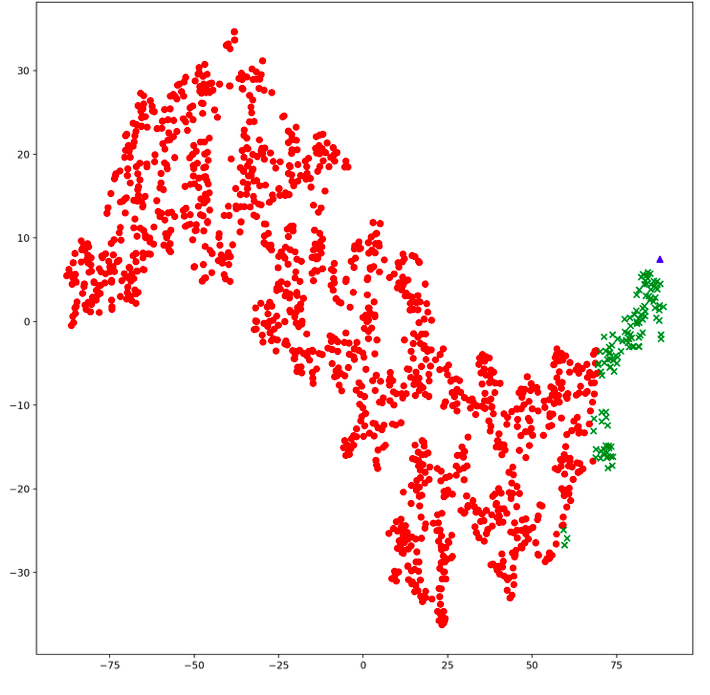
\includegraphics[width=0.5\textwidth]{images/Meanshift_Wine_22_5.png}
\end{center}
\caption{t-SNE projected result of Mean Shift with bandwidth = 22.5 on Red Wine Quality data set}
\label{fig:meanshift_wine_22_5}
\end{figure}
% \begin{itemize}
% \item What are the results and how are they measured?
% \end{itemize}

\subsubsection{Wine Quality - Affinity Propagation}
\textit{written by J.M.}\\

On the Wine Data set, Affinity Propagation works not good. The calculation to build cluster needs significantly longer because this data set has more data points than the other data sets. After it computes the clusters it builds many clusters. Figure \ref{fig:af_wine1} shows a plot of the clustering. There are many clusters in it. The parameter for this example was –6264. It does not work good for the same reason as for the House Pricing data set, because the dimensions are very high. The Silhouette Score is also low, only 0.32. 

\begin{figure}[H]
	\begin{center}
		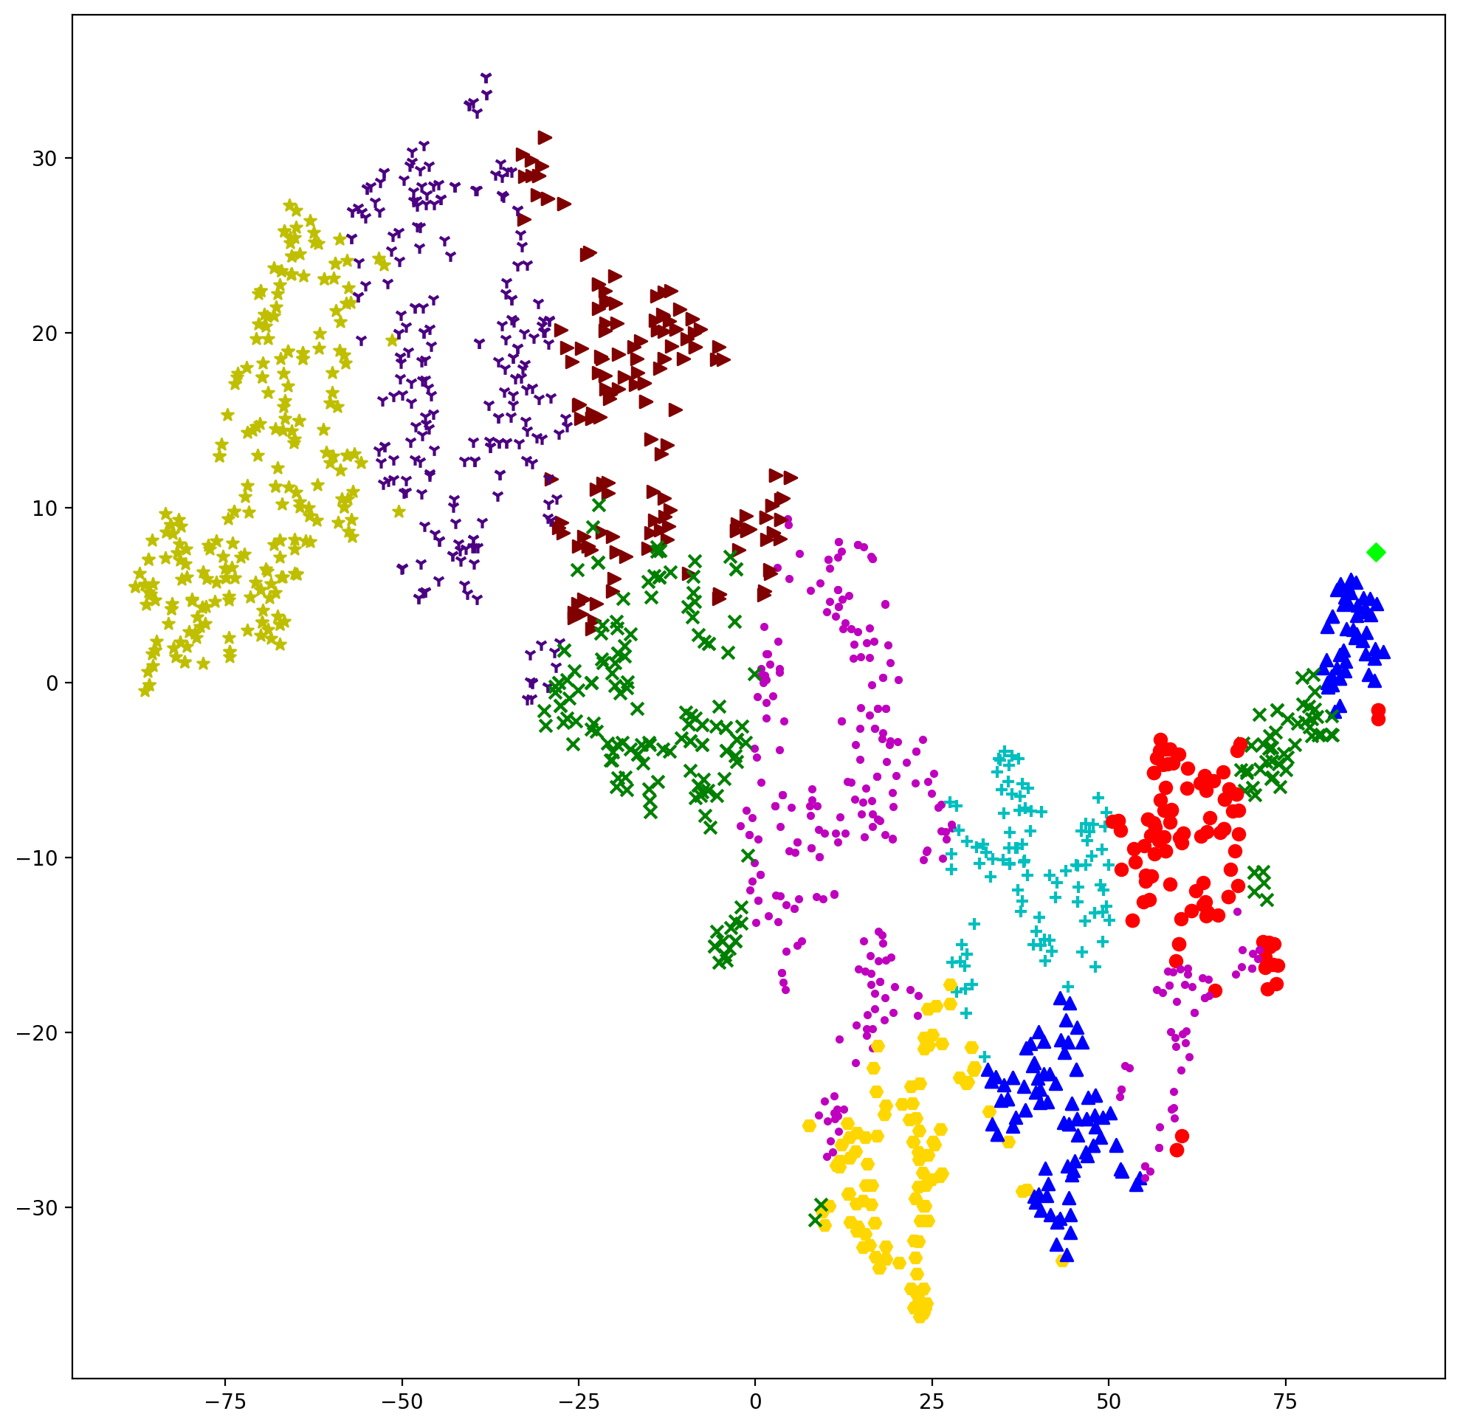
\includegraphics[width=0.5\textwidth]{images/af_wine6533.png}
	\end{center}
	\caption{t-SNE plot of Affinity Propagation on Wine Quality data set}
	\label{fig:af_wine1}
\end{figure}


\subsubsection{Wine Quality - Spectral Clustering}
\textit{written by M.A.}\\

The following table contains the index scores for each of the indices selected as columns and another column with the Parameter k. The values represent the maxima for CH, SI and DI and the minima for DB applied on the Wine Quality data set.\newline  
  


\begin{tabular}{lrrrrr}



{} &  Calinski-Harabasz &  Davies-Bouldin &  Silhouette &   Dunn &  Parameter k \\ \hline
0 &           2257.866 &           0.679 &       0.534 &  0.004 &          2 \\
1 &           2532.000 &           0.668 &       0.448 &  0.005 &          3 \\
2 &           2523.090 &           0.710 &       0.404 &  0.005 &          4 \\
3 &           2475.957 &           0.738 &       0.368 &  0.007 &          5 \\
4 &           2616.132 &           0.793 &       0.360 &  0.006 &          6 \\
5 &           2458.377 &           0.884 &       0.349 &  0.006 &          7 \\
6 &           2286.404 &           0.887 &       0.322 &  0.004 &          8 \\ \newline


\end{tabular}

Table 8: Spectral Clustering Data Set Indices by Number of Clusters.  \newline

\begin{figure}[H]
    \centering
    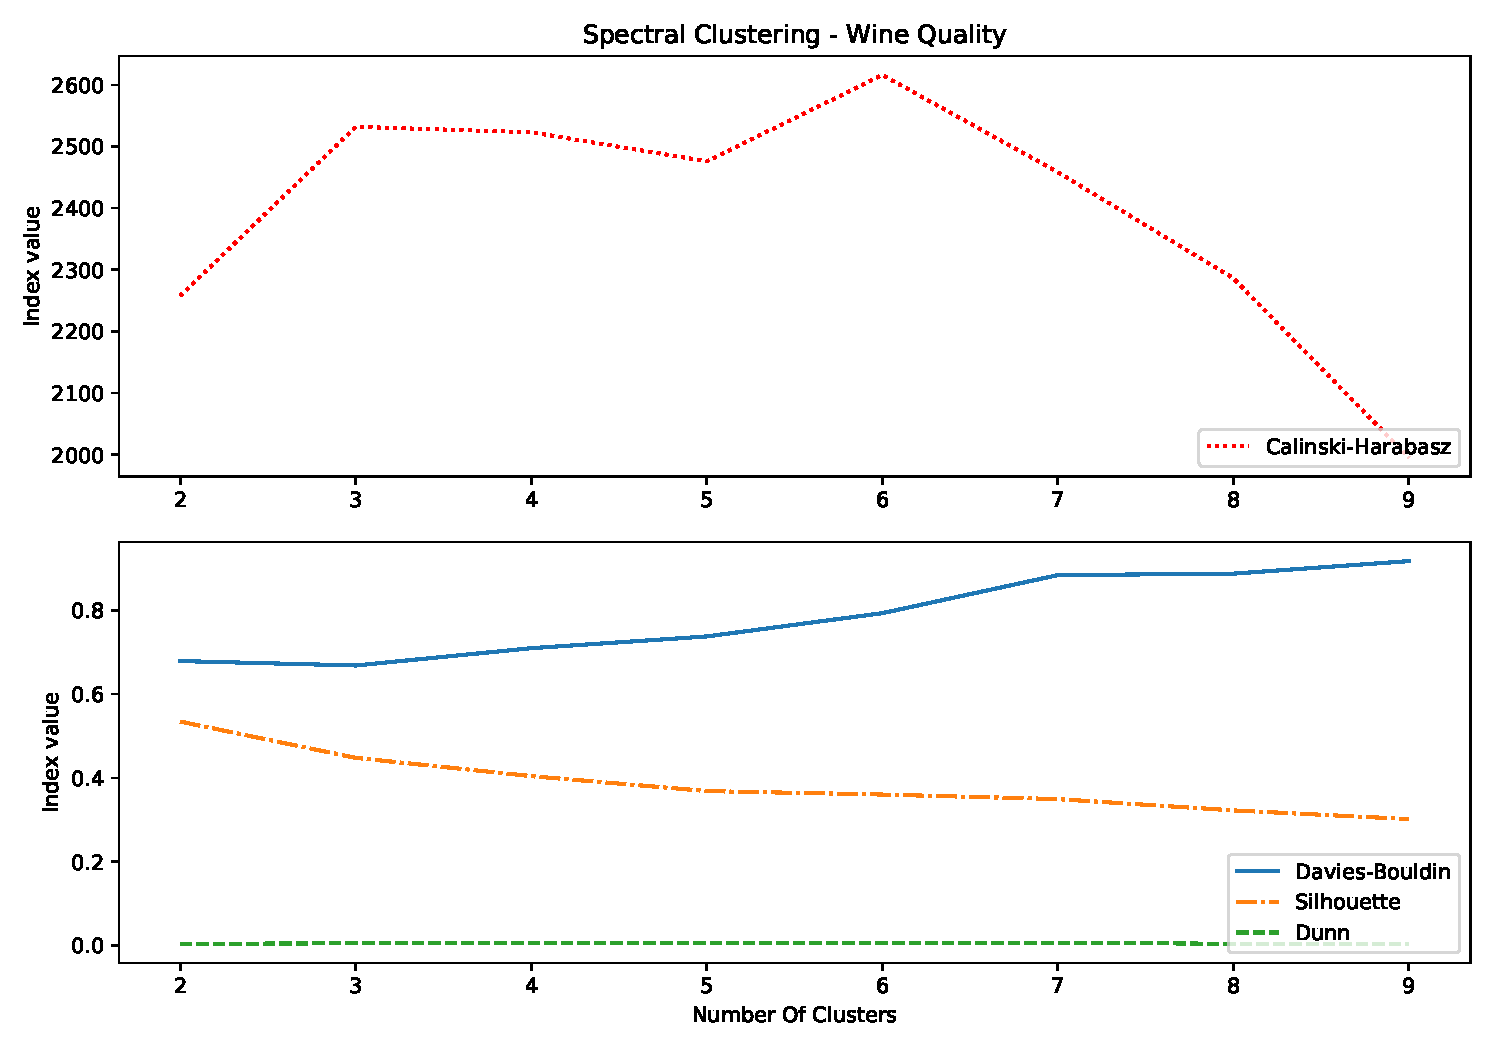
\includegraphics[width=1\textwidth]{images/Spectral_Clustering_-_Wine_Quality.pdf}
    \caption{Cluster validation indices by number of dimensions: Spectral Clustering on Wine quality data set}
    \label{fig:my_label323}
\end{figure}

In the Table 4 compared with Table 2 one can identify which dimension is the optimal, since the best values are already deposited in Table 4, but without the number of dimensions.
Analysing the table the maximal value for the Wine Quality data set with CH is being achieved with 6 clusters.\newline
Since the DB searches for the highest value to be a good index, the best cluster is being reached with  3 clusters. The maximum of SI is being reached with 2 clusters. The maximum of DI is reached while comparing the Index through 5 clusters, when compared with the big table. \newline
By the fact that, the Wine Quality data set is a big data set with many attributes and instances, it needed significantly longer than the other data sets. Nevertheless, the algorithm works correctly on the data set. \newline
